%%
%% This is file `sample-sigconf.tex',
%% generated with the docstrip utility.
%%
%% The original source files were:
%%
%% samples.dtx  (with options: `all,proceedings,bibtex,sigconf')
%% 
%% IMPORTANT NOTICE:
%% 
%% For the copyright see the source file.
%% 
%% Any modified versions of this file must be renamed
%% with new filenames distinct from sample-sigconf.tex.
%% 
%% For distribution of the original source see the terms
%% for copying and modification in the file samples.dtx.
%% 
%% This generated file may be distributed as long as the
%% original source files, as listed above, are part of the
%% same distribution. (The sources need not necessarily be
%% in the same archive or directory.)
%%
%%
%% Commands for TeXCount
%TC:macro \cite [option:text,text]
%TC:macro \citep [option:text,text]
%TC:macro \citet [option:text,text]
%TC:envir table 0 1
%TC:envir table* 0 1
%TC:envir tabular [ignore] word
%TC:envir displaymath 0 word
%TC:envir math 0 word
%TC:envir comment 0 0
%%
%% The first command in your LaTeX source must be the \documentclass
%% command.
%%
%% For submission and review of your manuscript please change the
%% command to \documentclass[manuscript, screen, review]{acmart}.
%%
%% When submitting camera ready or to TAPS, please change the command
%% to \documentclass[sigconf]{acmart} or whichever template is required
%% for your publication.
%%
%%
%% The Web Conference 2027 --- Research Track submission.
%% sigconf  : ACM two-column proceedings layout
%% review   : prints line numbers for reviewers
%% anonymous: suppresses the author block (double-blind review)
\documentclass[sigconf, review, anonymous, balance=false]{acmart}

%% --- Double-blind submission presentation (The Web Conference 2027) ---
%% Keep the ACM Reference Format block required by acmart for proceedings papers.
\settopmatter{printacmref=true}
%% 2) Remove the first-page footnote box that carries the copyright /
%%    permission notice, the conference line, the ISBN and the DOI. ACM
%%    populates these from the rights form at camera-ready time only; for
%%    review they must not appear.
\renewcommand\footnotetextcopyrightpermission[1]{}
%%
%% \BibTeX command to typeset BibTeX logo in the docs
\AtBeginDocument{%
  \providecommand\BibTeX{{%
    Bib\TeX}}}

%% Review submission: conference metadata is used for running headers only.
\acmConference[WWW '27]{Proceedings of The Web Conference 2027}{May 10--14,
  2027}{Dublin, Ireland}
\acmBooktitle{Proceedings of The Web Conference 2027 (WWW '27),
  May 10--14, 2027, Dublin, Ireland}
\copyrightyear{2027}
\acmYear{2027}
\acmDOI{}
\usepackage{xspace}
\usepackage{multirow}
\usepackage{subcaption}
\usepackage{booktabs}
%%
%% Submission ID.
%% Use this when submitting an article to a sponsored event. You'll
%% receive a unique submission ID from the organizers
%% of the event, and this ID should be used as the parameter to this command.
%%\acmSubmissionID{123-A56-BU3}
\newcommand{\ourmethod}{\textsc{BenchScout}\xspace}
\newcommand{\ptscpu}{PTS-CPU}
\newcommand{\ptsgpu}{PTS-GPU}
\newcommand{\id}[1]{{\itshape #1}}
\newcommand{\appname}{BenchScout}
\usepackage{xurl}
\newcommand{\sysctl}[1]{\texttt{\nolinkurl{#1}}}
%%
%% For managing citations, it is recommended to use bibliography
%% files in BibTeX format.
%%
%% You can then either use BibTeX with the ACM-Reference-Format style,
%% or BibLaTeX with the acmnumeric or acmauthoryear sytles, that include
%% support for advanced citation of software artefact from the
%% biblatex-software package, also separately available on CTAN.
%%
%% Look at the sample-*-biblatex.tex files for templates showcasing
%% the biblatex styles.
%%

%%
%% The majority of ACM publications use numbered citations and
%% references.  The command \citestyle{authoryear} switches to the
%% "author year" style.
%%
%% If you are preparing content for an event
%% sponsored by ACM SIGGRAPH, you must use the "author year" style of
%% citations and references.
%% Uncommenting
%% the next command will enable that style.
%%\citestyle{acmauthoryear}

%%
%% end of the preamble, start of the body of the document source.
\begin{document}

%%
%% The "title" command has an optional parameter,
%% allowing the author to define a "short title" to be used in page headers.
\title[\ourmethod]{\ourmethod: Compressing Cloud-Serving Evaluation with Execution-Anchored Sparse Probes}

%%
%% The "author" command and its associated commands are used to define
%% the authors and their affiliations.
%% Of note is the shared affiliation of the first two authors, and the
%% "authornote" and "authornotemark" commands
%% used to denote shared contribution to the research.


%%
%% By default, the full list of authors will be used in the page
%% headers. This command defines a more concise running header.
%% Kept anonymous to avoid leaking author identity during review.
\renewcommand{\shortauthors}{Anonymous Author(s)}

%%
%% The abstract is a short summary of the work to be presented in the
%% article.
\begin{abstract}
Benchmarking is central to cloud-infrastructure operations, where teams compare instances, detect regressions, and tune services. Yet comprehensive benchmark suites can take minutes or hours to run, making repeated evaluation costly in both time and shared compute resources. We observe that this breadth also creates redundancy: across benchmark components and Web workload levels, a small number of informative target-system measurements can anchor useful estimates of the complete profile. We present BenchScout, which uses host context to automatically select short, duration-bounded probes, executes them on the target system, and reconstructs unmeasured results from the observed anchors. We evaluate it on UnixBench and PTS-CPU across five Linux hosts, PTS-GPU on two hosts, and CloudSuite Web Serving. In run-held-out UnixBench evaluation, BenchScout achieves 0.21\% median suite-score error while reducing the estimated context-plus-probe budget from roughly 1,690\,s to 18.1\,s (about 99\%). On CloudSuite Web Serving, three measured load levels reduce cold-start throughput-curve MAPE from 39.16\% for history-only estimation to 7.21\% with adaptive selection and interpolation. These results show that automated, execution-anchored measurement can substantially reduce evaluation time while retaining accurate benchmark and Web performance profiles.

\end{abstract}

%%
%% CCS Concepts and keywords are mandatory for ACM proceedings
%% (including WWW). Generated from the tool at
%% http://dl.acm.org/ccs.cfm --- edit there and paste the result if needed.
%%
\begin{CCSXML}
<ccs2012>
   <concept>
       <concept_id>10011007.10011074.10011092</concept_id>
       <concept_desc>Software and its engineering~Software performance</concept_desc>
       <concept_significance>500</concept_significance>
   </concept>
   <concept>
       <concept_id>10010147.10010257.10010293</concept_id>
       <concept_desc>Computing methodologies~Machine learning~Machine learning approaches</concept_desc>
       <concept_significance>300</concept_significance>
   </concept>
   <concept>
       <concept_id>10011007.10011074.10011099</concept_id>
       <concept_desc>Software and its engineering~Software reliability</concept_desc>
       <concept_significance>100</concept_significance>
   </concept>
   <concept>
       <concept_id>10010520.10010575.10010755</concept_id>
       <concept_desc>Computer systems organization~Dependable and fault-tolerant systems and networks</concept_desc>
       <concept_significance>100</concept_significance>
   </concept>
</ccs2012>
\end{CCSXML}

\ccsdesc[500]{Software and its engineering~Software performance}
\ccsdesc[300]{Computing methodologies~Machine learning~Machine learning approaches}
\ccsdesc[100]{Software and its engineering~Software reliability}
\ccsdesc[100]{Computer systems organization~Dependable and fault-tolerant systems and networks}


%%
%% Keywords. The author(s) should pick words that accurately describe
%% the work being presented. Separate the keywords with commas.
\keywords{Web Infrastructure, HTTP Serving, System Benchmarking, Benchmark Suites, Performance Evaluation,
  Machine Learning, Sparse Measurement,
  Time-bounded Probing}
%% A "teaser" image appears between the author and affiliation
%% information and the body of the document, and typically spans the
%% page.


% \received{20 February 2007}
% \received[revised]{12 March 2009}
% \received[accepted]{5 June 2009}

%%
%% This command processes the author and affiliation and title
%% information and builds the first part of the formatted document.
\maketitle

\section{Introduction}
Benchmark suites~\cite{PTS,smith2011byte,kopytov2004sysbench} characterize modern computing platforms by running standardized workloads across processors, memory, storage, system software, and accelerators to produce a repeatable performance profile beyond any single measurement. They are widely used in performance-critical infrastructure workflows, including cloud instance comparison~\cite{aslanpour2020performance,lenk2011you,hwang2015cloud,marieska2011performance,moschetta2012ofbench,alhamazani2015cross}, monitoring~\cite{baruwal2016smart}, and performance autotuning~\cite{wang2023keentune,openeuler_atune_readme_zh,chen2024autoos,sun2025kconfigtune}. However, the same breadth that makes benchmark suites useful also makes them costly to execute in full. As Figure~\ref{fig:tuning_and_fullsuite_cost} illustrates, benchmark evaluation can dominate an auto-tuning task (Figure~\ref{fig:tuning_breakdown_pies}) and incur substantial wall-clock overhead across machine configurations (Figure~\ref{tab:fullsuite_execution_time}). Comprehensive suites combine heterogeneous workloads, each consuming time and competing for CPU, memory, storage, or accelerator resources. This cost compounds when measurements are repeated across machines, instance types, software revisions, and configurations.
\begin{figure}[t]
    \centering
    \begin{subfigure}[b]{0.46\linewidth}
        \centering
        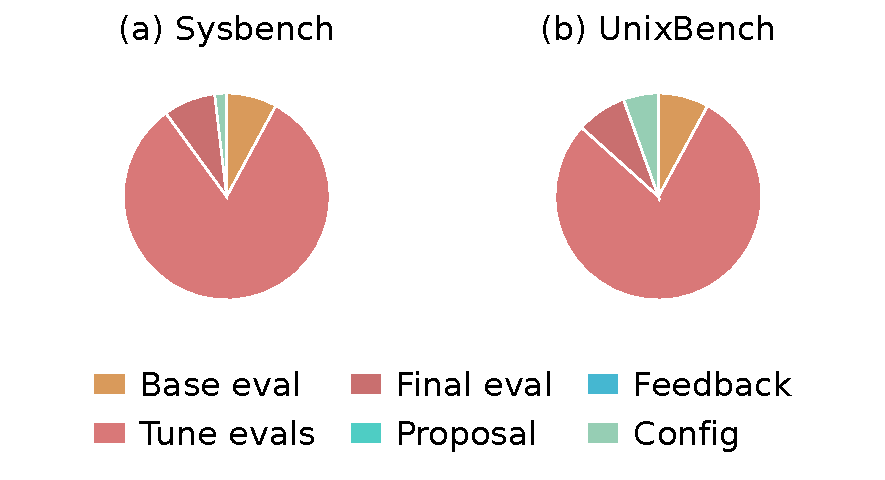
\includegraphics[width=\linewidth]{images/tuning_breakdown_pies_4x3.pdf}
        \Description{Two pie charts divide the runtime of representative KeenTune tasks among benchmark evaluation, tuning, proposal, feedback, and configuration stages.}
        \caption{Time breakdown of two representative KeenTune tasks.}
        \label{fig:tuning_breakdown_pies}
    \end{subfigure}
    \hfill
    \begin{subfigure}[b]{0.42\linewidth}
        \centering
        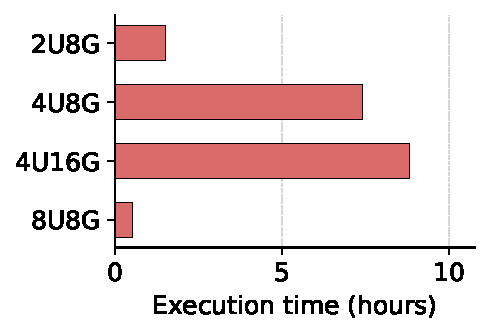
\includegraphics[width=\linewidth]{images/pts_cpu_runtime_bar.pdf}
        \Description{Horizontal bars compare full PTS-CPU execution times across five Linux hosts.}
        \caption{Full-suite PTS-CPU execution time across machines.}
        \label{tab:fullsuite_execution_time}
    \end{subfigure}
    \caption{Execution-time cost of benchmark-driven tuning and full-suite benchmark evaluation.}
    \label{fig:tuning_and_fullsuite_cost}
\end{figure}

Repeated evaluation amplifies this burden: autotuning revisits configurations, monitoring checks for regressions, and cloud users compare many candidate instances. BenchScout reduces this cost by automatically choosing a small number of informative measurements on the target system, bounding their duration, and reconstructing the remaining profile from those execution anchors. Unlike a fixed subset, the selected probes can respond to the host's measured context; unlike execution-free prediction, the estimates remain grounded in current target-system measurements.


% In the middle ground, execution-free predictors attempt to bypass benchmark runs by estimating performance from static host configurations, public specifications, or offline training data~\cite{wang2019predicting,tousi2022comparative}. 


% Because the system itself cannot magically compress the execution time of standard workloads, various approaches have attempted to mitigate this overhead. ``Static-subset'' approaches manually cherry-pick a fixed group of subtests, but they face a high barrier to generalization: a subset chosen for a CPU-bound instance falls short on an I/O-heavy machine~\cite{smith2011byte}. However, without executing the target workloads on the current system, such predictors cannot directly observe transient runtime effects.
% As a result, they can be unreliable under distribution shifts common in production environments.
% When a trustworthy performance profile is required, practitioners therefore still fall back to full-suite run-to-completion, preserving measurement fidelity at the cost of long delays and resource interference in shared environments.


% We take a different approach: rather than eliminating benchmark execution, \ourmethod keeps real measurements in the loop but makes them sparse and adaptive. 
% It reframes full-suite evaluation as conditional subset selection plus sparse reconstruction: under the current system state, \ourmethod observes only a small informative fraction of the suite and estimates the remaining official component scores and aggregate index.

% \paragraph{Problem scope and credibility.}
% \label{subsec:problem-scope}
% \ourmethod addresses two related but distinct needs.
% \textbf{(i)~Accelerated formal benchmarking:} autotuning, instance comparison, and regression testing repeatedly invoke standard suites and require estimates of the \emph{same} published indices ($Y=A(\mathbf{y})$) at far lower wall-clock and interference cost than run-to-completion execution.
% \textbf{(ii)~Fast performance portraits:} monitoring and capacity triage need a timely snapshot of how a host would likely score today, accepting approximation when a 30-minute full run is impractical.
% These modes impose different credibility bars.
% Accelerated formal benchmarking demands traceable sparse execution, per-host calibration against historical full runs, and explicit relative-error reporting against the full-run reference on the same host.
% Fast portraits tolerate higher approximation error but still require bounded probes, degradation-safe telemetry, and a fixed wall-clock budget that does not scale with suite cardinality.
% \ourmethod does \emph{not} claim to replace audited benchmark submissions; when certification matters---as with industrial SPEC submissions---its output is a preview and a run-to-completion execution remains the authoritative reference.

% \paragraph{Contributions.}
% \textbf{Systems:} \ourmethod is an end-to-end \emph{measurement pipeline}, not an execution-free score regressor.
% It (i)~binds every prediction to bounded real probes on the target host, (ii)~preserves official suite semantics ($\mathbf{y}$, $Y=A(\mathbf{y})$) rather than inventing surrogate metrics, (iii)~degrades gracefully when PMU/eBPF are blocked, and (iv)~reports fixed budgets ($K$, $T_{\mathrm{probe}}$) suitable for shared production hosts.
% \textbf{ML:} three supervised modules---conditional Top-$K$ router, prefix-to-score probe estimator, and masked reconstructor---are trained per host from historical full runs and composed in a single forward pass (Section~\ref{subsec:method-overview}).
% The router ranks experts by conditional informativeness; probe estimators map bounded telemetry to official component scores; the reconstructor imputes unobserved experts and the suite index from sparse tuples.
% ML selects \emph{which} experts to measure and \emph{how long} to probe; the OS executes the workloads and collects telemetry.
% We evaluate accelerated formal benchmarking (primary) and fast portraits (secondary) on five heterogeneous Linux hosts across UnixBench and PTS (Section~\ref{sec:evaluation}).

We make three contributions:
\begin{itemize}
    \item \textbf{Profile-preserving measurement compression.} We formulate evaluation as selecting target-system coordinates under a duration budget, then reconstructing the unmeasured components or load points so the output retains the diagnostic structure of a full profile.
    \item \textbf{A host-local suite pipeline.} BenchScout combines context-conditioned Top-$K$ routing, time-bounded component probes, and masked reconstruction to estimate suite components and an aggregate target while preserving the benchmark's published semantics.
    \item \textbf{Cross-workload accuracy--cost evidence.} Run-held-out UnixBench/PTS results and session-held-out CloudSuite results quantify profile fidelity alongside probe or phase cost. The evaluation spans component suites and multi-tier Web serving, with history, fixed, and adaptive controls that reveal how sparse measurement performs under stable and cold-start conditions.
\end{itemize}
These settings use different coordinates, split units, and estimators: run-held-out benchmark-suite profiles and session-held-out Web throughput curves. The Web study is a coordinate-specific instantiation of the same router--probe--reconstructor objective; its selector and reconstructor are specialized for offered-load curves, so we test role-level unity without claiming parameter-level transfer from UnixBench.



\section{Background and Motivation}

\subsection{Benchmark Suites and Web Profiles}

Benchmark suites provide reproducible and quantifiable measurements for comparing system performance across machines, configurations, and software versions. Rather than relying on a single workload, a suite decomposes system performance into multiple components, each targeting a distinct workload pattern across computation, memory, storage, networking, process control, and inter-process communication.
We denote a suite as \(\mathcal{B}=\{b_1,b_2,\ldots,b_N\}\), where \(b_i\) is the \(i\)-th component.
For a system state \(s\), the full result of component \(b_i\) is \(y_i=f_i(s,T_i,\epsilon_i)\), where \(T_i\) is the execution budget required by the original benchmark protocol and \(\epsilon_i\) denotes measurement noise; a full-suite run yields the result vector \(\mathbf{y}=[y_1,y_2,\ldots,y_N]\) and, when defined by the benchmark framework, an aggregate score \(Y=A(\mathbf{y})\).
Section~\ref{subsec:aggregator} instantiates $A(\cdot)$ for UnixBench and PTS.

The cost of full-suite benchmarking comes from two sources: the number of components and the duration of each component. Formally,
\begin{equation}
\label{eq:full-cost}
C_{\mathrm{full}}=\sum_{i=1}^{N}C_i(T_i).
\end{equation}
This cost can be substantial for suites with many components or long measurement intervals.
Practitioners invoke suites for two reasons with different credibility needs: repeated \emph{accelerated formal} evaluation that must approximate the same $Y$, and \emph{fast portraits} when a full run is infeasible.
However, not all observations are equally informative: components stress overlapping subsystems (Section~\ref{subsec:motivation-redundancy}), and prefix executions often expose the same rate trend as run-to-completion.
Our goal is therefore to estimate $(\mathbf{y},Y)$ from sparse, time-bounded probes while keeping real measurements in the loop: component estimates are either directly probed on the target host or reconstructed from probe-imputed partial observations. The aggregate target is the published UnixBench index for UnixBench and a paper-defined log-mean proxy for PTS.

The same representation applies to a Web service: for configuration $c$ and offered-load levels $\lambda_1,\ldots,\lambda_L$, its throughput profile is $\mathbf{q}_c=[q_c(\lambda_1),\ldots,q_c(\lambda_L)]$. The sparse-profile task selects a subset of coordinates under a preset duration cap for each target measurement, then estimates the remaining entries. A suite selects components; a Web workload selects offered-load levels. The endpoint and estimator are workload-specific even though the budgeted reconstruction problem is shared.


\subsection{Motivation}
% \paragraph{Observation 1: Full execution is expensive.}
% In Unix-like operating systems, we use UnixBench as a representative full-suite system benchmark. Originating from the BYTE UNIX benchmark suite, UnixBench remains a widely used open-source benchmark for evaluating system-level performance. It has been adopted in practical system tuning projects such as A-Tune~\cite{openeuler_atune_readme_zh} and KeenTune~\cite{wang2023keentune}. Figure~\ref{fig:tuning_breakdown_pies} reports the time breakdown of a typical KeenTune auto-tuning task. The results show that UnixBench evaluation dominates the overall tuning process, while the model tuning time accounts for only a small fraction. Since auto-tuning usually invokes the benchmark repeatedly to compare different configurations, the accumulated evaluation overhead quickly becomes unacceptable(Table~\ref{tab:fullsuite_execution_time}). Also, running the full suite consumes substantial system resources and can interfere with co-located applications. This makes full execution unsuitable for production-time detection.


% \paragraph{Observation 2: Full-suite scores are often unnecessary.}
% A full-suite benchmark usually aggregates the results of many heterogeneous components into a single overall score. However, for a specific workload or tuning objective, this aggregate score may not be the most meaningful optimization target. For example, a web service is usually more sensitive to request handling, process scheduling, networking, and memory behavior, while a compilation workload is more sensitive to process creation, filesystem activity, and CPU throughput. Optimizing the overall score may therefore waste measurements on components that have little relevance to the target workload, or even obscure the performance changes of the components that matter.

% \paragraph{Observation 3: Metrics converge before full completion.}
% Even when benchmark evaluation is needed, executing a selected component to completion is not always necessary. Many components are iterative rate tests rather than one-shot tasks. For example, Dhrystone and Whetstone in UnixBench~\cite{smith2011byte} repeatedly execute integer and floating-point operation kernels and report an operation rate. In these components, the final metric is computed from accumulated work over an execution interval. Therefore, a short prefix already contains direct information about the same rate that will be reported at the end of the full run. If the prefix rate becomes stable, continuing the benchmark mainly reduces statistical uncertainty rather than changing the measured quantity itself. This suggests that benchmark execution can be reduced vertically by estimating full-run metrics from short-run observations.

\paragraph{Motivation.}
\label{subsec:motivation-redundancy}
\label{subsec:motivation-convergence}
Suite components often share subsystem bottlenecks, while iterative rate tests expose useful signal before their full interval ends. We therefore test small fixed-duration selections against full references and matched history/fixed-subset controls. Optional PMU/eBPF telemetry is recorded with availability flags so missing counters do not change the feature schema (Section~\ref{subsec:feature-collection}); the detailed correlation and convergence diagnostics are reported in the supplementary artifact.




\section{Methods}
\label{sec:methods}

\begin{figure}
    \centering
    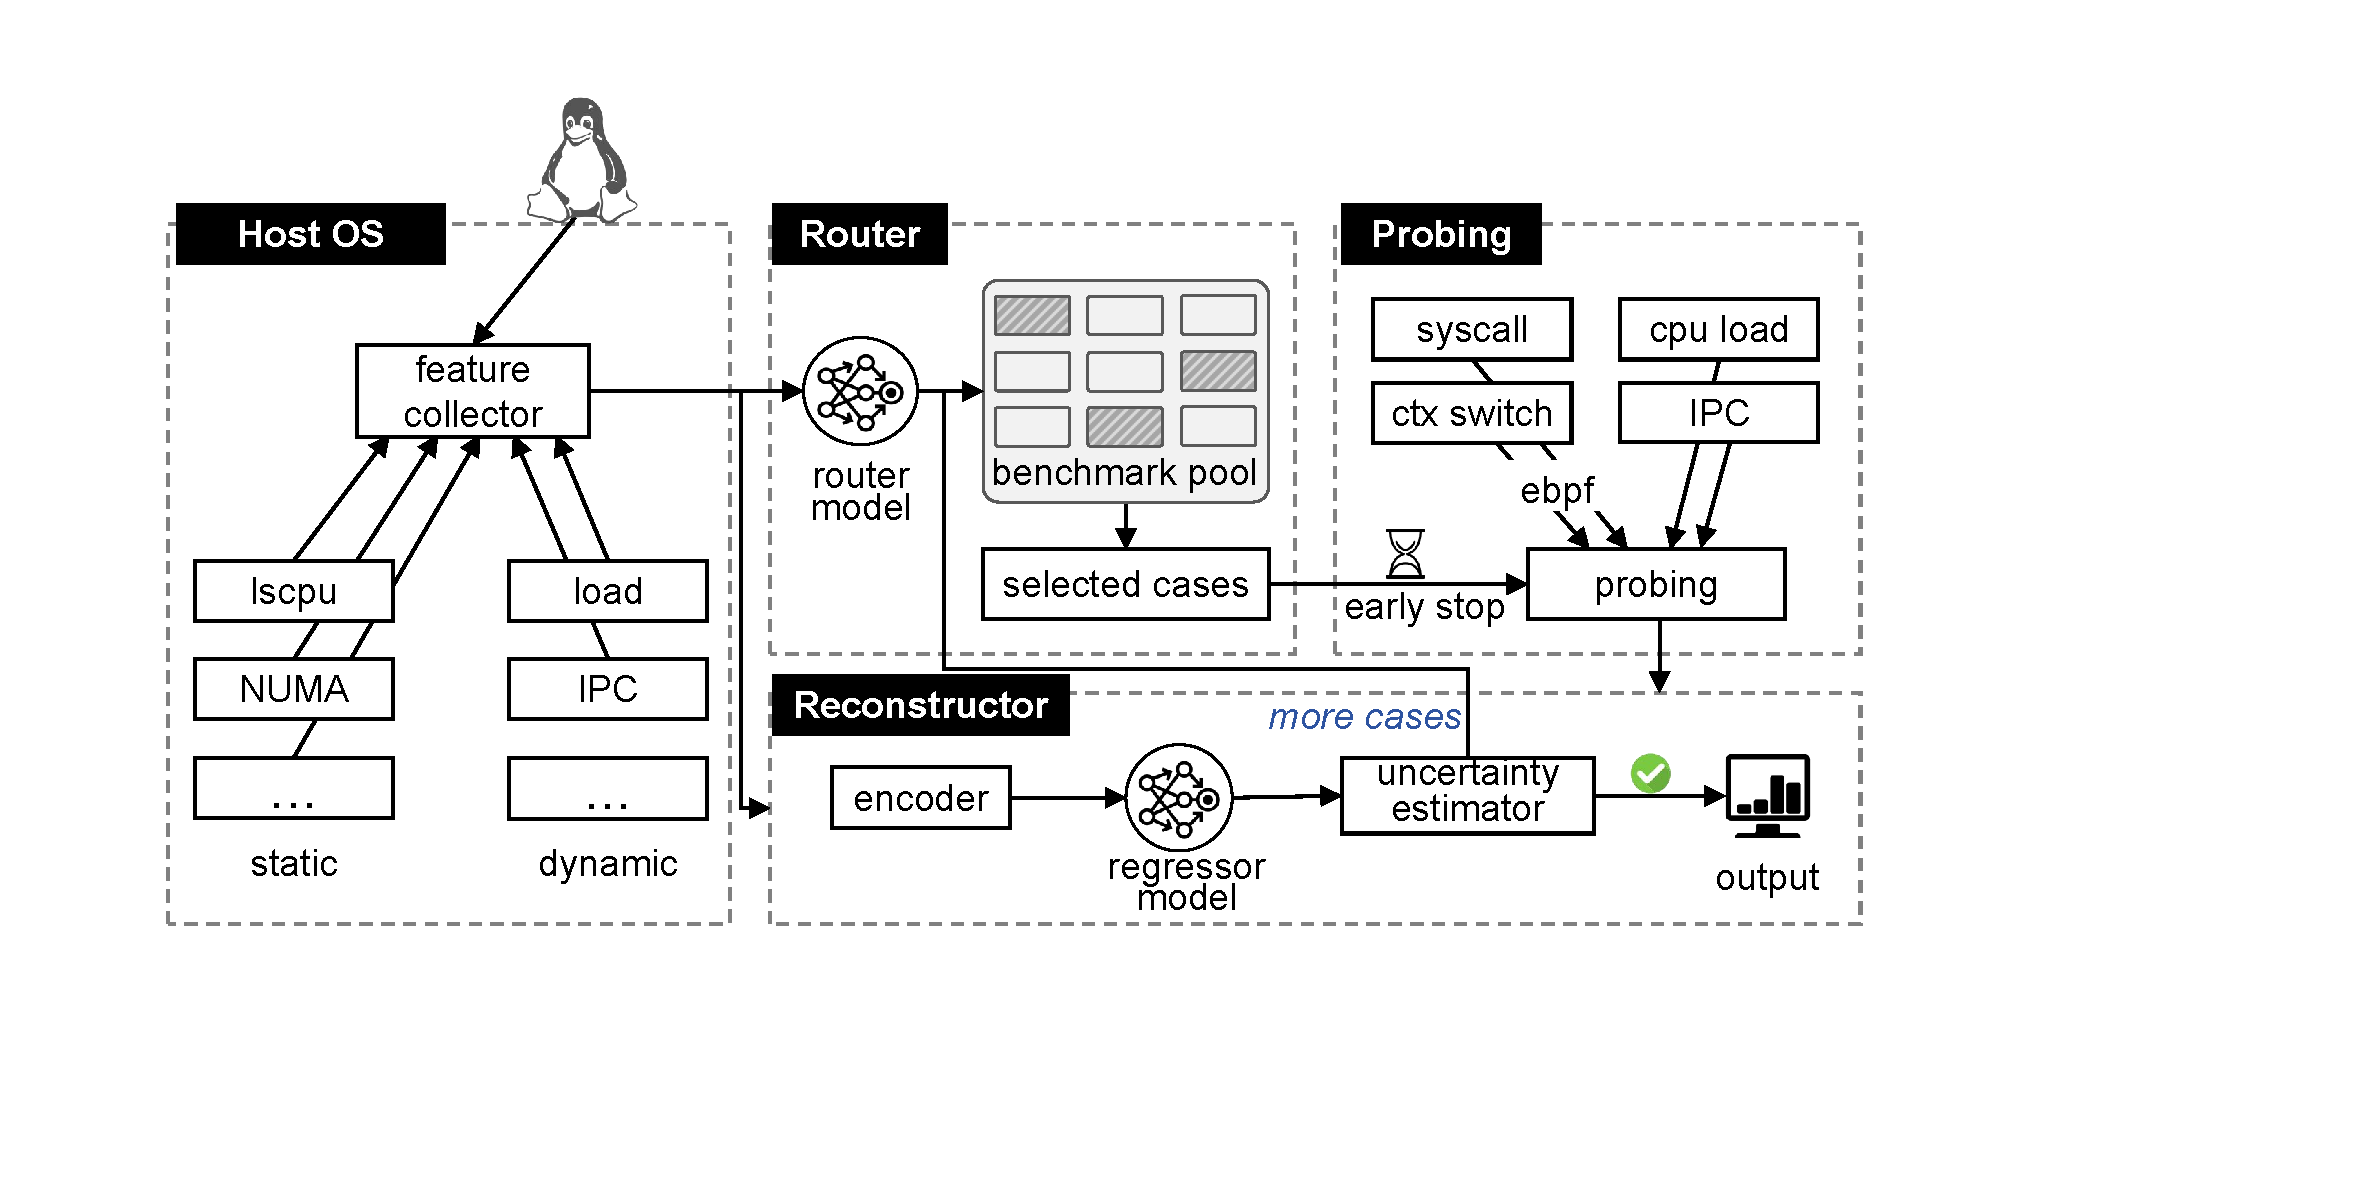
\includegraphics[width=1\linewidth]{images/mob.pdf}
    \Description{BenchScout pipeline: system context feeds a router, selected benchmarks run bounded probes, and a reconstructor estimates full-suite scores.}
    \caption{Overview of the \ourmethod architecture. (1)~\textbf{Host OS:} collector aggregates static and dynamic metrics into $\mathbf{x}$. (2)~\textbf{Router:} scores experts and selects Top-$K$. (3)~\textbf{Probing:} category micro-workloads (or real subtests) run under a fixed budget and emit $\mathbf{p}$. (4)~\textbf{Reconstructor:} multi-output regressor predicts $\hat{\mathbf{y}}$ and $\hat{Y}$.}
    \label{fig:mob}
\end{figure}


\subsection{Overview}
\label{subsec:method-overview}

\ourmethod approximates a complete benchmark run by observing only a small selected subset (Figure~\ref{fig:mob}).
Given the current system state, it collects context \(\mathbf{x}\), routes Top-$K$ subtests, runs fixed-duration probes on the selected components, and reconstructs the full official profile (Sections~\ref{subsec:router}--\ref{subsec:reconstructor}).
The pipeline is \emph{single-pass}: budgets ($K$, probe duration) are fixed at deployment; there is no adaptive re-probing loop.

\paragraph{Offline training and online protocol.}
\textbf{Offline}, each host $h$ collects $M$ complete runs $\{(\mathbf{x}_i,\mathbf{y}_i,Y_i)\}_{i=1}^M$ and trains a router $f_\theta$, probe estimators $f_{e_j}$, and a reconstructor $g_\phi$, persisting them as a host-local checkpoint bundle with no cross-host weight sharing.
\textbf{Online}, \ourmethod{} runs four deterministic stages: \textbf{Profile} $\mathbf{x}$ (3\,s warmup, 0.5\,s \path{/proc} sampling, perf PMU when permitted); \textbf{Route} the Top-$K$ experts via $f_\theta$; \textbf{Probe} each selected expert for a fixed $T_{\mathrm{probe}}$ (default 4\,s) to obtain $\hat{y}_j$; and \textbf{Reconstruct} the sparse tuple $Z=[\mathbf{x},m_j,\hat{y}_j,\tau_j]$ into $\hat{\mathbf{y}},\hat{Y}=g_\phi(Z)$.
The budget estimate is $T_{\mathbf{x}}+T_{\mathrm{selected\ probes}}$ (about 18\,s in the current hybrid artifacts, including a 3\,s context estimate and roughly 15\,s of selected probes) versus $C_{\mathrm{full}}$ (Equation~\ref{eq:full-cost}); unlike execution-free predictors~\cite{wang2019predicting,tousi2022comparative}, each prediction uses bounded on-host probes and per-host training. PTS suite comparisons use the proxy defined in Section~\ref{subsec:aggregator}.

\paragraph{Complexity and design invariants.}
The online cost is dominated by context collection and probing rather than model inference:
\begin{equation}
\label{eq:partial-cost}
C_{\mathrm{partial}} \approx T_{\mathbf{x}} + K \cdot T_{\mathrm{probe}} + T_{\mathrm{infer}},
\end{equation}
where $T_{\mathrm{infer}}$ is a sub-second tree/MLP forward pass and $T_{\mathbf{x}}$ is fixed regardless of suite cardinality $N$, whereas $C_{\mathrm{full}}$ scales with every component (Equation~\ref{eq:full-cost}).
This is a budget estimate; end-to-end wall time and interference must be measured for each deployment environment before operational use.

\subsection{Feature Collection and Engineering}
\label{subsec:feature-collection}

For run $i$, the pre-run context $\mathbf{x}_i=[\mathbf{x}_i^{\mathrm{static}},\mathbf{x}_i^{\mathrm{dynamic}}]$ combines stable host descriptors (CPU topology, NUMA layout, memory, OS/compiler versions) with transient pressure signals (utilization, iowait, load, runnable tasks, and perf/\path{/proc} counters).
Each probe of component $b_j$ yields a fixed-order prefix vector $\mathbf{p}_{i,j}$ containing progress and elapsed time, optional eBPF scheduling/syscall rates, \path{/proc} resource summaries, workload category, probe mode, and failure flags (Appendix~Table~\ref{tab:feature_collection}).
Unavailable dimensions are zero-filled with explicit availability flags, preserving a deterministic feature layout across training and inference.

\paragraph{Feature processing and dimensionality.}
\ourmethod uses domain-aware scaling rather than global MinMax/z-score normalization: static capacities keep physical magnitudes, dynamic counters become ratios or per-second rates, categorical and failure indicators are one-hot encoded, and missing values are zero-filled for deterministic inference.
When \texttt{perf}, eBPF, or GPU telemetry is unavailable, the collector records degradation flags and zero-masks affected dimensions instead of aborting. The context contains roughly 80--120 numeric capacity and pressure features.
This context/probe separation mirrors the Mixture-of-Experts pattern, in which a gating network conditions on global state while each expert observes task-local signals.


\subsection{Router: Conditional Expert Selection}
\label{subsec:router}

Because sub-benchmark outputs are correlated projections of the same system state (Section~\ref{subsec:motivation-redundancy}), a small diverse subset can suffice for full-suite reconstruction.
The selected subset is not fixed: the router's scores can vary with observed CPU, memory, and I/O context.
\ourmethod therefore treats benchmark acceleration as context-conditioned expert selection: given \(\mathbf{x}\), the router selects sub-benchmarks according to its learned score.

\paragraph{Expert Routing.}
Each executable sub-benchmark is a measurement expert in a fixed pool $\mathcal{E}=\{e_1,e_2,\ldots,e_n\}$.
Given \(\mathbf{x}\), a scoring model \(f_\theta\) assigns each expert a score \(s_i=f_\theta(\mathbf{x},e_i)\), which is normalized into a selection probability \(p_i=\exp(s_i)/\sum_{j=1}^{n}\exp(s_j)\).
The router then executes the Top-\(K\) experts \(\mathcal{S}_K(\mathbf{x})=\operatorname{TopK}_{e_i\in\mathcal{E}} p_i\), and the resulting partial observation vector is passed to the reconstructor to estimate the full-suite profile.

\paragraph{Training Objective.}
For each run $i$, all experts share context $\mathbf{x}_i$ and receive label $y_{i,j}$ from $\mathbf{y}_i$.
The LightGBM router minimizes a pairwise ranking loss using the within-run ordering of raw component scores; neural routers minimize cross-entropy to normalized component scores $\{y_{i,j}/\sum_k y_{i,k}\}$.
These objectives rank higher-scoring components; they do not directly optimize reconstruction error or the information gained by probing an expert.
Suite recovery is delegated to the reconstructor.
Budget $K$ trades accuracy for cost: smaller $K$ saves time but leaves fewer observations for reconstruction.

\paragraph{Router architectures and inference.}
We implement three router families: a \textbf{LightGBM ranker} treating each $(\mathbf{x}, e_i)$ pair as a ranking instance, and \textbf{MLP} and \textbf{GNN-expert} routers that embed $\mathbf{x}$ and emit a softmax-normalized logit vector $p_i$. Their supplementary model-grid comparison is retained in the experiment artifacts.
At inference the router selects the Top-$K$ experts by descending $p_i$, conditioned solely on pre-run context $\mathbf{x}$---never on probe outcomes---so the order Profile $\rightarrow$ Route $\rightarrow$ Probe $\rightarrow$ Reconstruct is preserved. In the audited corpus, each applicable host--suite pair has one collection session with five runs; this does not provide 15--60 independent labeled sessions.


\subsection{Time-Bounded Probing}
\label{subsec:time-bounded-probing}

Beyond horizontal subset selection, \ourmethod reduces per-expert cost via time-bounded probing: a fixed wall-clock window replaces run-to-completion execution, and a supervised estimator maps prefix telemetry to the official full-run score (Section~\ref{subsec:motivation-convergence}).

\paragraph{Dual-Mode Probing.}
\textbf{Micro-probes} map expert $e_j$ to a coarse category (CPU, memory, I/O, syscall, thread, GPU) and run a short synthetic stimulus (e.g., sqrt loop for \id{dhry2reg}, temp-file I/O for \id{fstime}) while collecting eBPF/\path{/proc} telemetry.
\textbf{Real-probes} invoke the original subtest under a hard timeout.
Both emit bounded telemetry $\mathbf{p}_{i,j}$ and predicted score $\hat{y}_{i,j}$; supervision always targets the official full-run label $y_{i,j}$.
Formally, for run $i$ and expert $e_j$, a per-expert estimator predicts $\hat{y}_{i,j}=f_{e_j}(\mathbf{p}^{\mathrm{micro}}_{i,j})$; in the shared-estimator setting, $\hat{y}_{i,j}=f(\mathbf{p}^{\mathrm{micro}}_{i,j},\mathrm{id}(e_j))$, where $\mathrm{id}(e_j)$ one-hot-encodes expert identity.
Production telemetry is often incomplete; \ourmethod encodes anomalies as features rather than discarding runs:
\begin{itemize}
    \item \textbf{Truncation:} timeout events set \id{real\_timed\_out} and record elapsed wall time.
    \item \textbf{eBPF fallback:} when tracing is unavailable, \id{ebpf\_available}${=}0$ and eBPF dimensions are zero-masked.
    \item \textbf{Rate normalization:} monotonic counters (\id{sched\_switch}, \id{syscall\_enter}) convert to per-second rates.
\end{itemize}

\paragraph{Parallel probe collection.}
Each probe runs three concurrent activities within the fixed wall-clock window $T_{\mathrm{probe}}$---an eBPF sampling thread (when permitted), the workload stimulus, and a trailing \path{/proc} snapshot---capturing kernel-level scheduling dynamics and user-space resource usage under the same budget rather than serializing telemetry after completion.
Real-probes invoke the benchmark subtest under a hard \texttt{timeout}, recording \id{real\_timed\_out} and elapsed wall time as features instead of aborting; the implementation defaults to micro-probes for predictable latency and supports real-probes when fidelity to the original binary path is required.

\paragraph{Training objective.}
The estimator minimizes $\mathcal{L}_{\mathrm{probe}}=\sum_{i,j}(\hat{y}_{i,j}-y_{i,j})^2$ in official label space (UnixBench indices; $\log(1+y)$-transformed PTS primaries), yielding fixed $T_{\mathrm{probe}}$ at inference.
Probe estimators are trained per host alongside the router and reconstructor; during \ourmethod{} inference, only the $K$ router-selected experts invoke live probes, while the remaining $n{-}K$ component scores are imputed exclusively by the reconstructor from the sparse tuple $Z$.


\subsection{Reconstructor: Full-Suite Result Recovery}
\label{subsec:reconstructor}

Given system context and sparse probe-imputed partial scores, the reconstructor is a multi-output regressor that predicts all unexecuted component scores and the aggregate suite index.
Its input deliberately interleaves global context $\mathbf{x}$ with per-expert tuples $(m_i,v_i,\tau_i)$ so that imputation can exploit both pre-run system state and which experts were actually probed, for how long, and with what estimated scores.

\begin{figure}
    \centering
    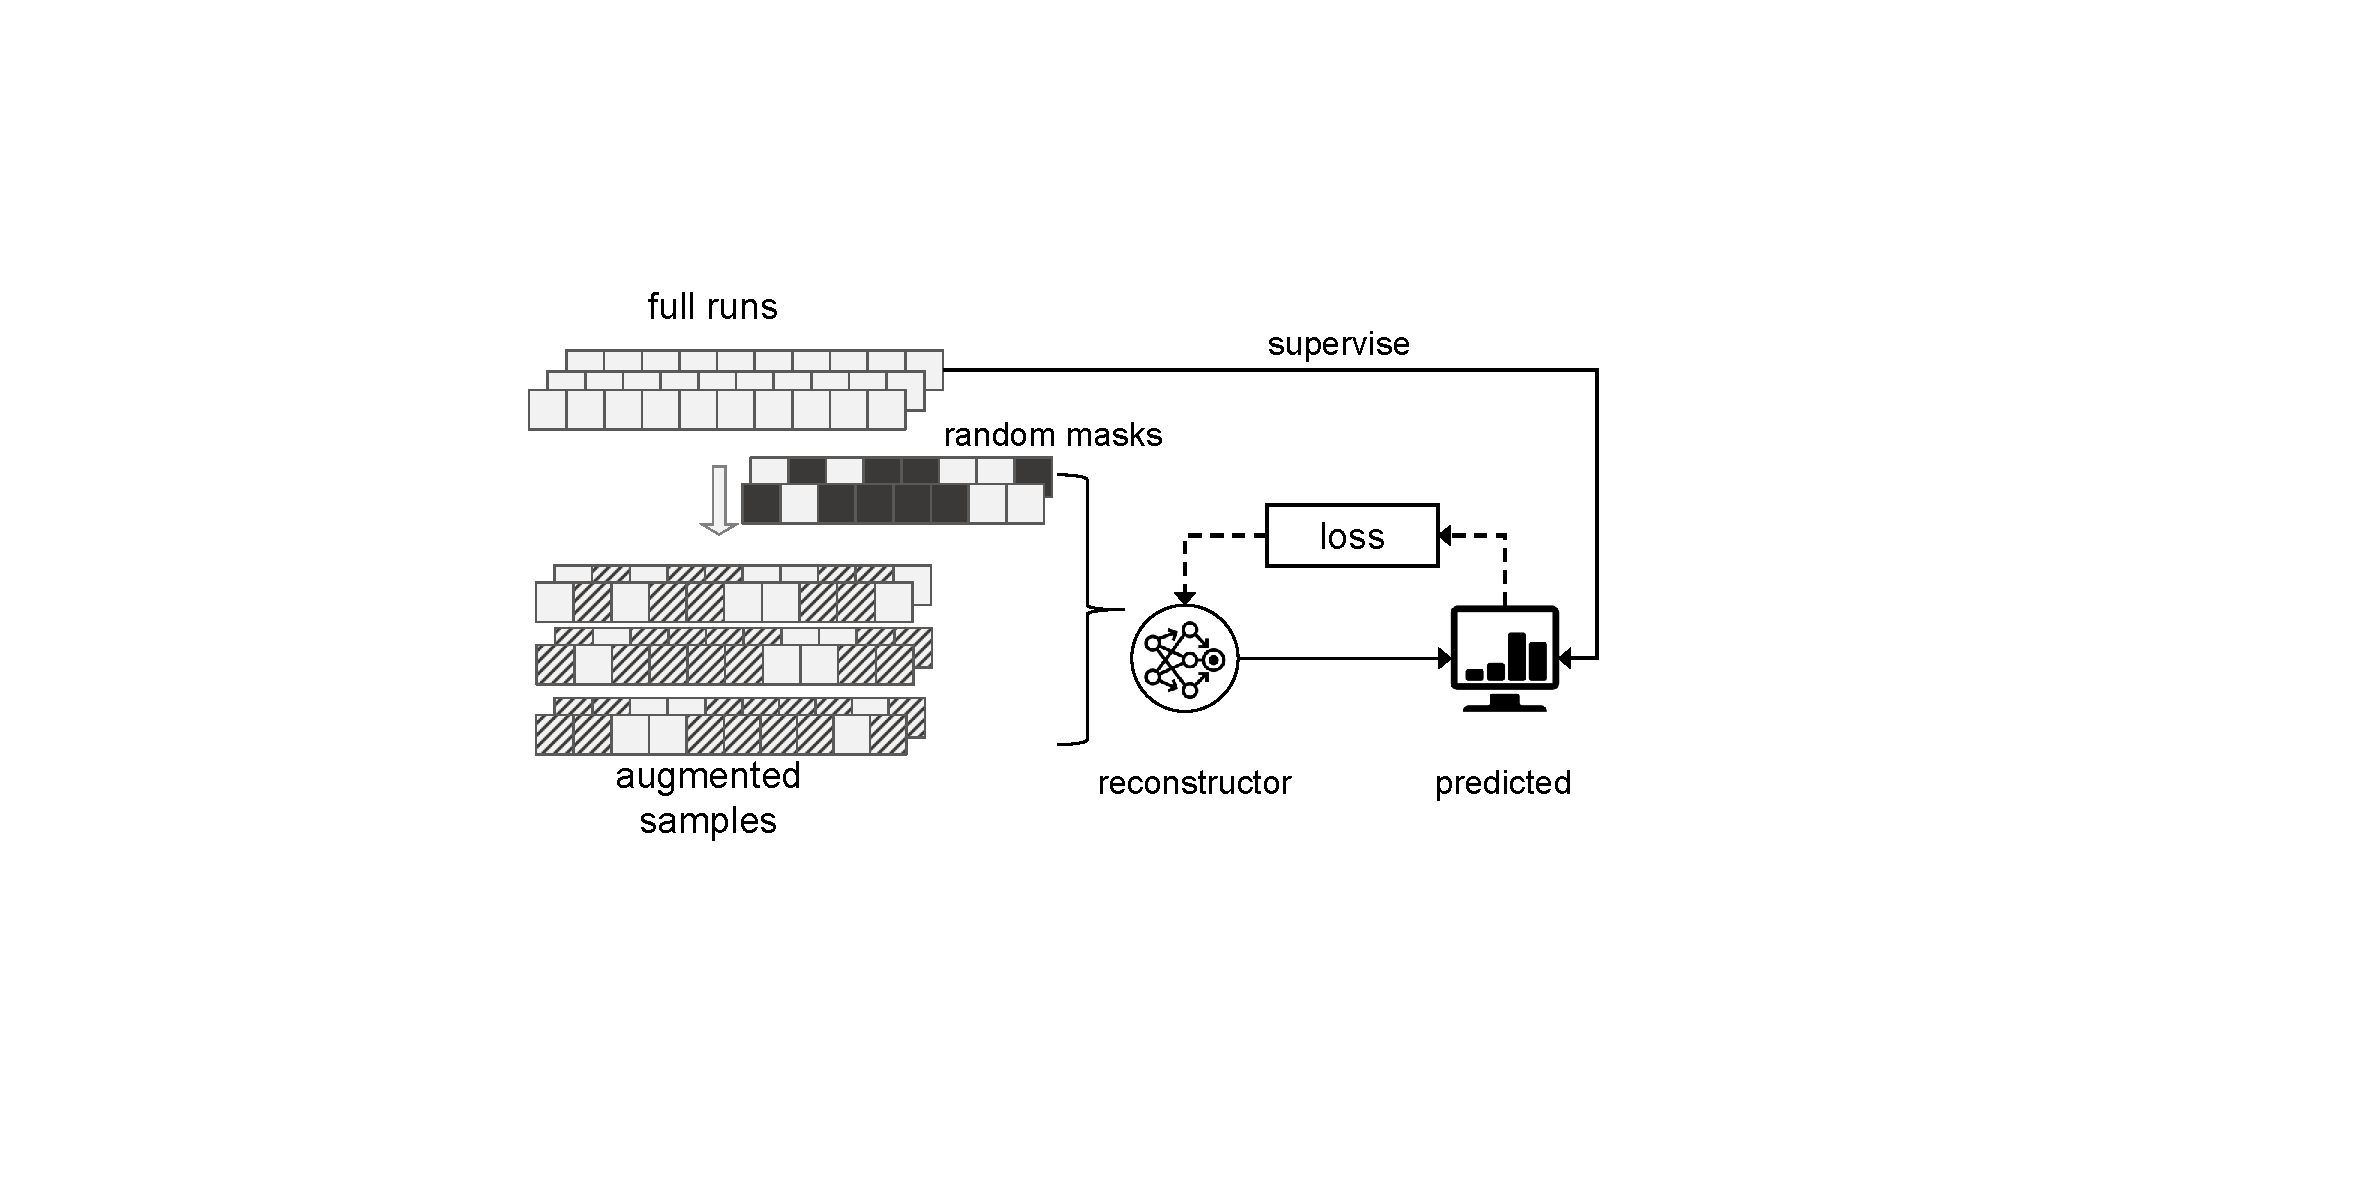
\includegraphics[width=1\linewidth]{images/recontruct.pdf}
    \Description{A reconstructor is trained on randomly masked historical full runs to predict the full benchmark result from sparse scores and a mask.}
    \caption{Reconstructor training with random-masked full runs. Historical full-run results are randomly masked to generate augmented sparse samples. The reconstructor takes the masked scores and binary mask as input, predicts the full-run result, and is optimized using the original full-run result as the supervision target.}
    \label{fig:reconstructor-training}
\end{figure}

\paragraph{Input Representation.}
Each expert $e_i$ is a 3-tuple \(z_i = (m_i, v_i, \tau_i)\) with mask $m_i$, score $v_i$, and probe wall time $\tau_i$ (zero-filled if unexecuted); the reconstructor input is the concatenation \(X=[\mathbf{x},z_1,\ldots,z_n]\).
Target \(Y = [r_1, \ldots, r_n, S]\) includes all component scores and suite index $S$; tree models use independent regressors per dimension.

\paragraph{Training and aggregation.}
\label{subsec:aggregator}
Historical full runs are augmented with random masks (Figure~\ref{fig:reconstructor-training}) and supervised with $\mathcal{L}_{\mathrm{recon}}=\|\hat{\mathbf{y}}-\mathbf{y}\|^2+(\hat{Y}-Y)^2$.
UnixBench labels use per-subtest \emph{Index} scores and the published \emph{System Benchmarks Index Score}.
For PTS, the profiles expose primary throughput or latency measurements but do not provide a single aggregate score used by this paper; we define a paper-specific proxy \(A_{\mathrm{logmean}}(\mathbf{v})=\exp(\frac{1}{N}\sum_{j=1}^{N}\log(1+v_j))-1\) over the included profile values.
This proxy is not an official PTS suite score. Probe and reconstructor inputs for PTS use $\log(1+y)$ scaling; the proxy is used as the PTS suite-level training and evaluation target.
The probe-only ablation, which has no reconstruction head, combines predicted UnixBench component indices using the smoothed geometric mean \(\exp(\mathrm{mean}_j\log(1+\hat{y}_j))-1\). This diagnostic aggregation differs slightly from UnixBench's published geometric mean of component indices; the full pipeline instead predicts the published suite index directly.

\paragraph{Mask augmentation and training input.}
The generic reconstruction path can augment historical full runs by randomly masking component scores (Figure~\ref{fig:reconstructor-training}): a random subset of size $k \sim \mathrm{Uniform}\{1,\ldots,n\}$ is marked observed ($m_i{=}1$, $v_i{=}y_i$), with unobserved entries set to zero.
This creates noiseless partial scores and does not itself model probe bias.
For the headline UnixBench hybrid OOF evaluation, the reconstructor instead trains on inner-fold out-of-fold probe predictions and their probe durations; outer-fold evaluation supplies predictions from the probe model fit on the outer training runs.
At inference, observed slots likewise carry probe-predicted scores $\hat{y}_j$ and measured durations $\tau_j$.
Tree-based reconstructors train one regressor per output dimension, handling heterogeneous score scales without shared output layers, while neural reconstructors use a shared trunk with multi-head outputs; both optimize the same $\mathcal{L}_{\mathrm{recon}}$ against official full-run labels.

\paragraph{End-to-end information flow.}
Figure~\ref{fig:mob} summarizes how the three modules compose: the router maps $\mathbf{x}$ to a discrete expert subset, probe estimators map prefix telemetry $\mathbf{p}_j$ to scores for observed experts, and the reconstructor maps the concatenated tuple $Z$ to the full vector $\hat{\mathbf{y}}$ and a separately predicted aggregate $\hat{Y}$.
The headline hybrid OOF protocol trains reconstruction on out-of-fold probe predictions, but the available evaluation does not establish that reconstruction reliably corrects probe bias; the random-mask training path uses noiseless observed scores.

\paragraph{Web curve instantiation.}
The Web specialization uses the same router--probe--reconstructor roles: the router selects offered-load coordinates, the probe is the real Faban cell, and the reconstructor fills omitted curve entries. The UnixBench probe-score model is not reused because Web cells already expose target throughput directly.
For Web profiles, the coordinates are five offered-load levels, with a budget of $K=3$ target measurements capped at 60\,s each. The nested selector evaluates all ten three-load subsets by inner session-held-out curve MAPE using training sessions only. The adaptive selector starts at the lowest offered load and greedily adds the load maximizing $|\hat{z}_j|\,s_{j\mid S}$, where $\hat{z}_j$ is the correlation model's predicted standardized deviation from the training mean and $s_{j\mid S}$ is the conditional standard deviation given the already selected loads $S$. The correlation estimator uses training-fold means, scales, and correlations; matched controls use linear interpolation with endpoint extrapolation or least-squares scaling of the training-fold mean curve. Sessions remain the split unit, and cold-start folds train on the other PHP-FPM setting. This is the Web workload adapter of the same budgeted-profile objective: its selector and estimator are specialized to ordered load curves, whereas the suite implementation selects benchmark components and predicts their scores.


\section{Evaluation}
\label{sec:evaluation}

\subsection{Experimental Setup}
\label{subsec:exp-setup}

% We evaluate \appname{} on five heterogeneous Linux hosts.
% UnixBench and \ptscpu{} run on all five audited machines; supplied \ptsgpu{} values cover M1 and M6.

% Our primary method is the integrated \ourmethod{} pipeline.
% We collect $\mathbf{x}$ once, use a router to select Top-$K$ sub-benchmarks, run a short probe (default 4\,s) on \emph{only} those selected components, and reconstruct the full-suite score from probe-predicted partial observations.
% Ground-truth scores and wall times come from previously collected complete runs on the same host (offline replay); we do \emph{not} re-execute full suites during \ourmethod{} evaluation.

% We exhaustively compare all $3 \times 2 \times 3 = 18$ router--probe--reconstructor combinations on each applicable host--suite pair.
% \emph{Router only} (Top-$K$ \emph{full} partial execution + reconstruction) and \emph{probe only} (probe \emph{all} components without reconstruction) are retained as ablation baselines.
% Unless stated otherwise, each host trains and evaluates only on its own collected runs.

% Main-experiment and supplementary tables report measured values over five audited CPU hosts and supplied GPU values for M1/M6.
% Values are aggregated from per-host offline cross-validation JSON under \path{dataset/paper_supplementary/}.

% \subsubsection{Testbeds}
% \label{subsubsec:testbeds}
\paragraph{Testbeds.}
The audited CPU corpus contains five Linux host identities (Table~\ref{tab:testbeds}), referred to by the compact CPU$\times$RAM shorthand used throughout this section. The GPU comparison also includes the supplied M6/NVIDIA T4 result; CPU and memory specifications for M6 were not reported.
M1 (32 vCPU, Intel Core i9-14900K, 128\,GiB, NVIDIA RTX 3090\,Ti) and M6 (NVIDIA T4) have available GPU comparison values; M2--M5 are CPU-only in the audited corpus (Intel Xeon 6982P-C or Xeon Platinum).


\begin{table}[t]
\centering
\caption{Testbeds represented in the evaluation. M1--M5 are the audited Linux CPU corpus; M6 is included for its supplied NVIDIA T4 GPU result. M6 CPU and RAM specifications were not reported.}
\label{tab:testbeds}
\small
\setlength{\tabcolsep}{2pt}
\begin{tabular}{@{}lp{0.36\linewidth}rc@{}}
\toprule
\textbf{Host} & \textbf{vCPU (CPU model)} & \textbf{RAM} & \textbf{GPU} \\
\midrule
M1 & 32(Intel Core i9-14900K) & 128GB & NVIDIA RTX 3090 Ti GPU \\
M2 & 2(Intel Xeon 6982P-C) & 8GB & --- \\
M3 & 4(Intel Xeon 6982P-C) & 8GB & --- \\
M4 & 4(Intel Xeon 6982P-C) & 16GB & --- \\
M5 & 8(Intel Xeon Platinum) & 8GB & --- \\
M6 & Not reported & Not reported & NVIDIA T4 GPU \\
\bottomrule
\end{tabular}
\end{table}


\paragraph{Feature collection.}
System context $\mathbf{x}$ is collected with a 3\,s warmup and 0.5\,s \path{/proc} sampling; when perf PMU counters are blocked the collector falls back to \path{/proc}-based proxies without aborting, and GPU dimensions are zero-masked on CPU-only hosts---mirroring the degradation paths of the online pipeline (Section~\ref{subsec:feature-collection}).



\paragraph{Benchmark suites.}
\label{subsubsec:benchmark-suites}
We use three suites that stress complementary subsystems.
\textbf{UnixBench} (UB) is a classic system-level suite with $N{=}12$ single-copy subtests spanning CPU kernels, filesystem I/O, and OS/interaction workloads; its aggregate is the \emph{System Benchmarks Index Score}.
\textbf{PTS-CPU} adds $\approx$13 compilation, cryptography, compression, and numerical profiles. We report their primary throughput or latency metrics and use the paper-defined log-mean proxy from Section~\ref{subsec:aggregator} for suite-level comparisons.
\textbf{PTS-GPU} adds OpenCL/GPU compute workloads.
UnixBench and PTS-CPU run on M1--M5 in the audited raw corpus; available PTS-GPU comparison values cover M1 and M6. The audited raw CPU and M1 GPU corpus has one collection session of five runs for each applicable host--suite pair; the supplied M6 comparison has no accompanying run-count metadata here.

\paragraph{Web-serving workloads.}
We additionally evaluate two HTTP workloads, which are separate from the UnixBench/PTS host--suite corpus. The multi-tier CloudSuite Web Serving workload uses PHP, MySQL, and Memcached with Faban as the load generator on M1; its profile has five offered-load levels and two PHP-FPM settings (\texttt{max\_children}=4 and 8). The strict curve analysis uses four valid held-out sessions per setting after excluding the session with a failed transaction, with session-level splits. A separate static-content Nginx workload runs on M1 over loopback, comparing \texttt{worker\_processes}=1 and 4 at five offered loads in four randomized blocks (80 completed cells). The two HTTP workloads are reported separately because CloudSuite measures a multi-tier application while Nginx provides a lightweight static-content counterexample. Their collection and split protocols are detailed in Sections~\ref{subsec:http-pilot} and~\ref{subsec:nginx-counterexample}.

\paragraph{Baselines.}
The \emph{full-run} baseline executes the entire suite and serves as the reference.
The zero-probe train-fold mean is a same-host history baseline. Fixed-first, fixed-middle, and random subsets test how much a selected subset matters; router-only replays compare policies when selected component scores are known. We also evaluate two local execution-free proxies inspired by Wang et al.~\cite{wang2019predicting} and Tousi et al.~\cite{tousi2022comparative}. These DNN and MLP implementations use the available static hardware features and are not reproductions of the cited methods, so they do not support conclusions about those method families.
All predictive baselines use the same reported within-session folds. The execution-free proxies incur feature-collection cost ($\approx$3.5\,s), while \ourmethod{} adds bounded probes. Since each host--suite has one five-run session, these comparisons do not test temporal or session-level generalization.


%%%
% 多一组1685s 

% \paragraph{Why UnixBench and PTS, not SPEC CPU2017.}
% SPEC CPU2017 is the industrial processor reference, but our target workflows---cloud auto-tuning, regression testing, and operator monitoring---need open, scriptable suites that exercise CPU, I/O, OS, and GPU subsystems without license-managed publication.
% We evaluate on UnixBench and PTS accordingly; certified SPEC submission lies outside our scope.

\paragraph{Evaluation protocol.}
We evaluate three execution paths---the \ourmethod{} pipeline (main method: collect $\mathbf{x}$, router Top-$K$, probe the selected components, reconstruct the suite score), a \emph{router-only} ablation that substitutes \emph{measured} partial scores on the routed subset for probe predictions, and a \emph{probe-only} ablation that probes every component without routing or reconstruction---plus supplementary studies on Top-$K$, features, telemetry, and probe duration.
Every raw host--suite pair available to this study consists of one session with five runs. The reported cross-validation is a within-session random-fold analysis; folds contain very few test samples, and the repository audit found no machine-readable manifest for a locked train/validation/test split or session-level holdout. Thus model selection and generalization beyond these runs cannot be independently established from the available corpus. Models are fit separately per host, so these results do not measure cross-host transfer.
Full-run labels and wall times come from previously collected runs, so the headline evaluation is an offline replay. Partial times in that analysis are budget estimates unless explicitly identified as online measurements.

% Table~\ref{tab:overall-effectiveness-cpu} reports the primary \ourmethod{} path.
% For each held-out test run, we replay the pre-run context $\mathbf{x}$ and probe telemetry $\mathbf{p}$; the router selects a Top-$K$ subset, the probe estimator produces probe-imputed component scores $\hat{\mathbf{y}}$, and the reconstructor outputs the aggregate prediction $\hat{Y}$.
% The partial scores given to the reconstructor are always \emph{probe-imputed} scores on the router-selected subset, never measured partial scores taken from the full-run JSON.
% We compare $\hat{Y}$ against the reference aggregate score $Y$ from the same run to compute suite-level relative error.

% This offline protocol avoids re-executing thousand-second full suites.
% The held-out test runs were collected 24 hours after the training corpus, providing a time-separated evaluation rather than contemporaneous replay.
% Section~\ref{subsec:resource-waveforms} corroborates wall-time savings with online traces.
% \emph{Router-only} ablations substitute measured partial scores and must not be conflated with \ourmethod{} headline numbers.



% \paragraph{Per-host training protocol.}
% For every host from M1 to M5, we collect benchmark datasets locally and train all models using only runs whose session tags match that host.
% M1 trains and evaluates on UnixBench, \ptscpu, and \ptsgpu; M2--M5 train and evaluate on UnixBench and \ptscpu{} only.
% This isolates each machine's router, reconstructor, and probe models from other hosts' data distributions.
% Cross-host comparison therefore reflects how \appname{} behaves under different hardware ceilings rather than a single global model transferred across machines.


% For \ourmethod{} and \emph{router only} end-to-end grid experiments on PTS, ground-truth full-suite scores are taken from previously collected full runs on the same host (offline replay), avoiding repeated full-suite online execution that can cause excessive wall time or resource exhaustion.
% \ourmethod{} UnixBench evaluation likewise replays historical runs for accuracy and uses dataset-recorded full-suite wall times for cost comparison.

% \subsubsection{Collected Data}
% \label{subsubsec:collected-data}

% \paragraph{Phase~1: Full-suite collection (shared by all routes).}
% On each host, we collect multiple complete benchmark sessions (typically 3--5 rounds per session) for every suite applicable to that host.
% UnixBench and \ptscpu{} sessions are collected on all five audited hosts; supplied \ptsgpu{} values cover M1 and M6.
% Each run record stores system context $\mathbf{x}$, per-component results $\mathbf{y}$ and timings $\mathbf{t}$, and expert metadata (component identifiers, categories, and titles).
% These runs provide supervision for router training, reconstructor training, probe label construction, and ground-truth evaluation.

% \paragraph{Phase~2: \ourmethod{} main experiment (router + probe + reconstruct).}
% For each applicable suite on each host, we train three router architectures (LightGBM ranker, MLP, GNN-expert), three reconstructors (XGBoost, LightGBM, MLP), and two probe regressors (LightGBM and XGBoost).
% We evaluate all $3 \times 2 \times 3 = 18$ \ourmethod{} combinations offline.
% For each historical run, the router selects Top-$K$ components, probe predictions substitute for executed subtest scores on the selected subset only, and the reconstructor predicts the suite score.
% Partial wall time is estimated as $\hat{T}_{\mathrm{xi}} + K \cdot T_{\mathrm{probe}}$ (default $\hat{T}_{\mathrm{xi}}=3$\,s, $T_{\mathrm{probe}}=4$\,s); full-suite wall time is read from the dataset.

% \paragraph{Phase~3: Ablation --- \emph{router only} (partial full execution + reconstruction).}
% We repeat the \(3 \times 3\) router--reconstructor grid using \emph{actual} partial sub-benchmark execution scores (not probe predictions) on the router-selected subset, matching the original \emph{router only} design.

% \paragraph{Phase~4: Ablation --- \emph{probe only} (probe all components).}
% For each applicable suite on each host, we build a probe dataset by executing short probes (default 4\,s per component, micro-probe mode) over historical full runs on the same host, train two regressors (LightGBM and XGBoost), and evaluate suite prediction by probing \emph{every} component and aggregating---without router selection or reconstruction.

% \paragraph{Phase~5: Supplementary offline studies (\emph{router only} best combination).}
% After selecting the best router--reconstructor pair per suite from Phase~2 on each applicable host, we conduct three supplementary studies on stored runs only (leave-one-session-out cross-validation, no re-execution):
% Top-$K$ sweep, routing-policy comparison, and system-feature ablation.
% For \ptsgpu, supplementary studies use M1 data only.


% \subsection{Data Collection and Training Protocol}
% \label{subsec:data-and-protocol}

% To ensure rigorous evaluation and prevent data leakage across heterogeneous hardware environments, we enforce a strict per-host protocol for both data collection and model training.

% \paragraph{Full-Suite Data Collection.}
% For every host from M1 to M5, we construct a local ground-truth dataset by executing multiple complete benchmark sessions (typically 3--5 full rounds per session) for every suite applicable to that host.
% Specifically, UnixBench and \ptscpu{} sessions are collected across all five machines, while \ptsgpu{} sessions are collected exclusively on M1.
% During each full-suite execution, the system records a comprehensive profile containing the pre-run system context $\mathbf{x}$, per-component score results $\mathbf{y}$, component execution timings $\mathbf{t}$, and associated expert metadata (e.g., component identifiers and workload categories).
% These complete historical runs serve as the foundational dataset, providing necessary supervision for router training, reconstructor targets, probe label construction, and final ground-truth evaluation.

% \paragraph{Per-Host Training Isolation.}
% We treat each machine as an independent operational environment.
% For every host, all models (including routers, reconstructors, and probe estimators) are trained using \emph{only} the runs whose session tags match that specific host.
% This design strictly isolates each machine's pipeline from the data distributions of others.
% Consequently, our cross-host evaluation reflects how \appname{} adapts to different hardware ceilings autonomously, rather than relying on a single, globally transferred model.

% \paragraph{Offline Replay for Evaluation.}
% Evaluating large-scale, comprehensive suites via repeated online execution incurs excessive wall-clock time and introduces unmanageable resource exhaustion and thermal throttling variances.
% To mitigate this, our end-to-end evaluations (including the \ourmethod{} pipeline and ablation grids) adopt an offline replay methodology.
% For both PTS and UnixBench experiments, ground-truth full-suite scores and wall times are extracted directly from the previously collected datasets.
% During validation, the system simulates the partial execution by retrieving the corresponding sub-benchmark records, ensuring a statistically sound and highly reproducible cost comparison without the overhead of redundant physical executions.

\paragraph{Metrics.}
\label{subsubsec:metrics}
We report the suite relative error $|\hat{S}-S|/\max(|S|,\epsilon)$, where $\hat{S}$ is produced entirely by model inference and the reference index $S$ serves only as the label, and the saved wall-time fraction $f_{\mathrm{saved}}=(T_{\mathrm{full}}-T_{\mathrm{partial}})/T_{\mathrm{full}}$.
For Top-$K$ comparison we use a balanced score (lower is better) that prioritizes accuracy and treats time savings as a tie-breaker,
\begin{equation}
\label{eq:balanced-score}
\mathrm{Bal} \;=\; \frac{e}{e_{\min}} \;+\; \lambda \,(1 - f_{\mathrm{saved}}),
\end{equation}
where $e$ is the mean out-of-fold suite relative error, $e_{\min}=\min e$ across the compared settings, and $\lambda = 0.15$.
Feature-ablation importance is the relative-error increase $\Delta e_m=(e_m-e_{\mathrm{full}})\times 100$ percentage points when group $m$ is removed.

\subsection{System-Suite Profile Results}
\label{subsec:overall-effectiveness}

Table~\ref{tab:overall-effectiveness-cpu} reports five-fold run-held-out estimates from the historical corpus: five held-out runs per host--suite, or 25 predictions per suite across five hosts. Each fold fits the router, probe estimator, and reconstructor on the other four runs; reconstructor inputs are probe-estimator outputs $\hat{y}_j$, not measured scores from the held-out run. Fold-local LightGBM reconstructors use 30 estimators for PTS and 200 for UnixBench.

BenchScout achieves 0.21\% median UnixBench suite-index error at an estimated 18.1\,s context-plus-probe budget, comprising about 3\,s of context collection and 15.1\,s of selected probes. On the same 25 held-out runs, its 300 component predictions have 0.86\% mean relative error (4.34\% at the 95th percentile); restricting the denominator to the 225 unselected components gives 0.88\% mean MAPE across runs. The corresponding omitted-component means are 2.29\% for PTS-CPU (140 components over 25 runs) and 2.48\% for the five-run M1 PTS-GPU audit. Full-suite times come from representative historical runs, so the table does not report paired end-to-end speedups. The static-feature proxies are local implementations, not reproductions of the cited methods.

The train-fold mean is a warm-start control that uses other runs from the same host--suite session and requires no new measurement. BenchScout has lower point error on 3/5 UnixBench hosts and 2/5 PTS-CPU hosts; history is at least as accurate on the others. These are within-session estimates, and the reported time values combine nominal probe budgets with historical full-run times rather than paired end-to-end measurements.

For M1 UnixBench, additional selective-execution controls (Section~\ref{subsec:selective-execution-baselines}, Table~\ref{tab:m1-strong-baselines}) show that subset selection and reconstruction can work well with measured component scores. These replay baselines and adaptive probing use different information or cost accounting, so they are not matched end-to-end competitors to probe-imputed \ourmethod{}.

We also ran the four policies online on the current M1 host, rather than replaying archived probe records. One complete single-copy UnixBench run supplied a common live reference (index 1816.3; 1,720.9 s), followed by three randomized repetitions in which each policy collected three fresh 4-second micro-probes. Table~\ref{tab:matched-routing} reports these measurements. The live reference ran under the concurrent host load recorded in the artifact, so this is a validation of the deployed pipeline under that operating condition, not a replacement for the within-session OOF estimate. The online predictions are much higher than the reference (75.77\% mean error) and nearly identical across policies, exposing a temporal/load shift that the historical checkpoint does not absorb.

For comparison, the archived five-host OOF replay gives 0.590\% mean error for all four policies and identical per-run suite predictions on the 25 held-out runs. This is a genuine null result, not duplicated measurements: the fold-local reconstructors map policy-specific partial inputs to the same suite estimate. A feature-use audit found zero probe-feature split gain in 22 of 25 suite-output heads, consistent with the reconstructor relying predominantly on host context for this target. The fold-matched context-only control has 0.608\% mean error. Thus the historical folds show no accuracy advantage for learned routing, while the new online run reveals poor temporal/load robustness.

\begin{table}[t]
\centering
\caption{Live UnixBench routing-policy comparison on M1. One complete single-copy reference run (index 1816.3; 1,720.9 s) was followed by three randomized repetitions of fresh online micro-probes per policy. Each row averages three repetitions; learned selections vary by repetition. Probe wall is the sum of selected process wall times, while phase wall includes collection overhead. The host was concurrently loaded; raw probes, load averages, affinity, and reference report are in the artifact JSON.}
\label{tab:matched-routing}
\scriptsize
\setlength{\tabcolsep}{3pt}
\begin{tabular}{lrrrr}
\toprule
\textbf{Policy} & \textbf{Mean prediction} & \textbf{Mean err. (\%)} & \shortstack{\textbf{Probe wall}\\\textbf{(s)}} & \shortstack{\textbf{Probe phase}\\\textbf{(s)}} \\
\midrule
Learned Top-$3$ & 3192.429 & 75.766 & 15.087 & 15.228 \\
Fixed first-$3$ & 3192.429 & 75.766 & 15.066 & 15.290 \\
Fixed CPU-mix & 3192.429 & 75.766 & 15.070 & 15.439 \\
Fixed I/O-mix & 3192.429 & 75.766 & 15.100 & 15.230 \\
\bottomrule
\end{tabular}
\end{table}

\paragraph{Interpretation.} In the live run, all policies produce nearly the same prediction despite selecting different components; the current reconstructor is insensitive to the fresh probe values under this shifted operating state. The online result is therefore a measured robustness failure, not evidence that the policies are equivalent in general. The archived OOF audit likewise found zero probe-feature split gain in 22/25 suite-output heads and no accuracy advantage from learned routing. We retain both views because the historical folds and live deployment answer different questions.

\begin{table*}[t]
\centering
\caption{Overall effectiveness on CPU benchmark suites across five heterogeneous CPU hosts (M1--M5).
\ourmethod{} rows use the full pipeline: router Top-$K$, \emph{probe-model-predicted} partial scores, and reconstruction (Section~\ref{subsec:overall-effectiveness}).
Wang-style DNN and Tousi-style MLP rows are local execution-free proxies inspired by~\cite{wang2019predicting,tousi2022comparative}, using static hardware features only; they are not reproductions of the cited methods.
PTS-CPU proxy errors use the same log-mean targets and run-held-out folds as \ourmethod{}. Time is an estimated new-measurement budget in seconds: zero for history, about 3.5\,s for static-feature collection, and 18.0--18.1\,s for BenchScout context plus selected probes. Full-suite entries are historical wall times, not paired timing controls. Bold marks the lowest error in each host column.}
\label{tab:overall-effectiveness-cpu}
\footnotesize
\setlength{\tabcolsep}{3.2pt}
\begin{tabular}{llcccccccccc}
\toprule
\multirow{2}{*}{\textbf{Suite}} & \multirow{2}{*}{\textbf{Method}} & \multicolumn{2}{c}{\textbf{M1 (32U128G)}} & \multicolumn{2}{c}{\textbf{M2 (2U8G)}} & \multicolumn{2}{c}{\textbf{M3 (4U8G)}} & \multicolumn{2}{c}{\textbf{M4 (4U16G)}} & \multicolumn{2}{c}{\textbf{M5 (8U8G)}} \\
\cmidrule(lr){3-4} \cmidrule(lr){5-6} \cmidrule(lr){7-8} \cmidrule(lr){9-10} \cmidrule(lr){11-12}
& & \textbf{Err. (\%)} & \textbf{Time (s)} & \textbf{Err. (\%)} & \textbf{Time (s)} & \textbf{Err. (\%)} & \textbf{Time (s)} & \textbf{Err. (\%)} & \textbf{Time (s)} & \textbf{Err. (\%)} & \textbf{Time (s)} \\
\midrule

\multirow{5}{*}{UnixBench} 
& Full-suite & -- & 1691.0 & -- & 1520.0 & -- & 1580.0 & -- & 1610.0 & -- & 1550.0 \\
& Train-fold mean & 0.21 & 0.0 & \textbf{0.19} & 0.0 & 0.35 & 0.0 & \textbf{0.13} & 0.0 & 2.78 & 0.0 \\
& Wang-style DNN proxy & 0.21 & 3.5 & 2.67 & 3.5 & 6.28 & 3.5 & 4.47 & 3.5 & 4.37 & 3.5 \\
& Tousi-style MLP proxy & 1.7 & 3.5 & 99.56 & 3.5 & 99.63 & 3.5 & 99.60 & 3.5 & 99.59 & 3.5 \\
& \ourmethod & $\mathbf{0.18}$ & 18.1 & 0.29 & 18.1 & $\mathbf{0.34}$ & 18.1 & 0.19 & 18.1 & $\mathbf{1.95}$ & 18.1 \\

\midrule

\multirow{5}{*}{\ptscpu} 
& Full-suite & -- & 15755.0 & -- & 12450.0 & -- & 13100.0 & -- & 13900.0 & -- & 12800.0 \\
& Train-fold mean & 1.91 & 0.0 & \textbf{0.16} & 0.0 & \textbf{0.18} & 0.0 & \textbf{0.21} & 0.0 & 0.22 & 0.0 \\
& Wang-style DNN proxy & 1.91 & 3.5 & 0.26 & 3.5 & 68.53 & 3.5 & 0.22 & 3.5 & \textbf{0.17} & 3.5 \\
& Tousi-style MLP proxy & 1.88 & 3.5 & 99.42 & 3.5 & 99.93 & 3.5 & 97.57 & 3.5 & 98.77 & 3.5 \\
& \ourmethod & $\mathbf{1.74}$ & 18.0 & 0.19 & 18.1 & 0.26 & 18.0 & 0.30 & 18.0 & 0.19 & 18.0 \\

\bottomrule
\end{tabular}
\end{table*}



\paragraph{PTS-GPU results.} Table~\ref{tab:pts-gpu-audited} reports a five-run, one-session M1 comparison on the paper-defined log-mean target; history and the static DNN proxy have lower error than the fold-based hybrid estimate (0.9534\%). A separate online report gives 0.18\% for M1 and 0.14\% for M6/T4 at a reported 15\,s. These values use a different protocol: M1's held-out target overlaps model selection and the 15.03\,s probe time excludes 7.93\,s context collection; M6 run-level logs are unavailable. We retain them as provenance-only case-study values in Appendix~\ref{app:artifact-notes}, separate from the fold comparison.

\begin{table}[t]
\centering
\caption{M1 PTS-GPU run-held-out comparison on the paper's log-mean target (five runs, one session). All rows use the same held-out runs. History mean uses the other four training labels; execution-free proxies use static hardware features; BenchScout uses host context and selected probes. Cost is the estimated new measurement budget, not model-training or end-to-end serving time.}
\label{tab:pts-gpu-audited}
\tiny
\setlength{\tabcolsep}{1.5pt}
\begin{tabular}{lrr}
\toprule
\textbf{Method} & \textbf{Mean err. (\%)} & \textbf{Cost (s)} \\
\midrule
Train-fold history mean & 0.7993 & 0 \\
Wang-style DNN proxy & \textbf{0.7987} & 3.5 \\
Wang-style linear proxy & 0.8492 & 3.5 \\
Tousi-style random forest & 0.8695 & 3.5 \\
Tousi-style decision tree & 0.8492 & 3.5 \\
Tousi-style MLP & 0.8592 & 3.5 \\
Tousi-style elastic net & 0.8298 & 3.5 \\
\ourmethod{} full pipeline & 0.9534 & 18.0 \\
\bottomrule
\end{tabular}
\end{table}

The supplied online GPU comparison is kept distinct from the run-held-out table: M1's target run was included in the model-selection corpus, and the T4 run-level logs are unavailable. The 15-second figure is selected-probe time; M1 adds 7.93 seconds of context collection, for 22.965 seconds total hybrid wall time. These measurements are useful as concrete case studies on two GPU hosts, but they are not independent estimates of generalization.

\begin{table}[t]
\centering
\caption{Supplied online PTS-GPU case studies. Values are separate from run-held-out results: the M1 target overlaps model selection and M6/T4 logs are unavailable. Cost denotes selected-probe time; M1 context collection adds 7.93\,s.}
\label{tab:gpu-provenance}
\footnotesize
\setlength{\tabcolsep}{4.5pt}
\begin{tabular}{llcc|cc}
\toprule
\multirow{2}{*}{\textbf{Suite}} & \multirow{2}{*}{\textbf{Method}} & \multicolumn{2}{c|}{\textbf{M1 (RTX 3090 Ti)}} & \multicolumn{2}{c}{\textbf{M6 (T4)}} \\
\cmidrule(lr){3-4} \cmidrule(lr){5-6}
& & \textbf{Err. (\%)} & \textbf{Cost (s)} & \textbf{Err. (\%)} & \textbf{Cost (s)} \\
\midrule
\multirow{4}{*}{\ptsgpu}
& Full-suite & -- & 27018.0 & -- & 12951.0 \\
& Wang-style DNN proxy & 0.26 & 3.5 & 5.13 & 3.5 \\
& Tousi-style MLP proxy & 98.85 & 3.5 & 67.14 & 3.5 \\
& \ourmethod & $\mathbf{0.18}$ & 15.0 & $\mathbf{0.14}$ & 15.0 \\
\bottomrule
\end{tabular}
\end{table}

\subsection{Transfer and Temporal Diagnostics}
\label{subsec:transfer-diagnostics}
The in-corpus folds estimate within-session interpolation, so we separately inspect one later M1 run and an offline host-held-out replay. These diagnostics ask whether the learned policy travels beyond the rows used to fit it; they are not pooled into the headline accuracy estimates.

On 2026-10-12, checkpoints saved on June 10 or earlier predicted 3189.654 for a newly collected M1 UnixBench run whose full-run target was 3418.5 (6.6943\% error, $n=1$). Router scores tied across all 12 subtests, triggering the implementation's directory-order fallback to \id{dhry2reg}, \id{whetstone-double}, and \id{execl}. Context collection took 8.699\,s and the three real probes took 3.012\,s. This temporal observation shows a material gap between excellent within-session folds and a later run; the tied router and single observation preclude a generalization claim. The records also show a scikit-learn 1.8.0-to-1.7.2 checkpoint compatibility warning.

In an offline leave-one-host-out replay, test hosts were excluded from router, probe-model, and reconstructor fitting; source-host reconstruction used inner host-held-out probe fits. Probes were archived from full-run collections rather than freshly executed on the held-out hosts. The four compared policies average 15.07\% mean host error and 40.44\% worst-host error, with mean errors within 0.002 percentage points of one another; predicted suite indices differ by at most 0.079 over 25 runs. Thus host transfer remains difficult, and current evidence does not show the learned policy improving over alternatives under host shift.

An oracle subset diagnostic isolates the value of choosing components when their full-run scores are already known. A training-host score-ranked subset has 4.49\% mean error (0.98--10.25\% across hosts), versus 9.53\% for random, 12.57\% for first-three, 16.26\% for context-only Ridge, and 22.60\% for training mean. This indicates that target-host component observations can be informative, but it is an upper-bound diagnostic: it does not validate pre-run routing, short probes, or online transfer.

\subsection{Multi-tier CloudSuite Web Profile}
\label{subsec:http-pilot}
CloudSuite Web Serving is a multi-tier application with PHP, MySQL, and Memcached; all tiers and the Faban load generator run on M1 over a private Docker bridge. We compare PHP-FPM \texttt{max\_children}=4 and 8 over five offered-load levels, with four independently restarted sessions per configuration. Each session contains 60-second probe cells and 120-second full-reference cells with fresh services between cells. We hold out a complete session and fit selectors and curve estimators on the other three; the session, not an individual load cell, is the evaluation unit. A session enters the strict primary analysis only if all 20 configuration, phase, and load cells are present, have valid operation mixes, and have no failed transactions. Sessions 1, 2, 4, and 5 pass this rule. Session 3 has one failed Register transaction and is excluded from the primary analysis; it is retained only in a separately labeled one-failure sensitivity analysis. The locked split is recorded in the session-audit JSON under the round-8 results directory (input hash prefix \texttt{ff3bc3c19b75}; the full hash is in the artifact). This CloudSuite instantiation uses workload-specific load selection and sparse-curve reconstruction to measure the accuracy--cost trade-off directly; its selector and estimator are analyzed as a distinct Web workload component of the measurement-compression study.

For this CloudSuite/Faban workload, operation-level latency limits are p95 $\leq$ 500\,ms and p99 $\leq$ 1,000\,ms. We report these as a workload-specific feasibility screen separate from the primary throughput-profile fidelity endpoint; they are not a general prerequisite for the system-suite experiments.

Every probe policy receives the same three 60-second load measurements per configuration. The primary same-configuration analysis trains and tests on the same PHP-FPM setting using different sessions. A separate cold-start analysis transfers estimates from the other setting and measures curve error only; it is not used to claim a configuration-choice result. We report the two transfer directions separately because their profile shapes differ. Controls include training-session history, nested and adaptive selection, fixed first/middle/evenly spaced loads, interpolation, history scaling, and the exact expectation over all ten random three-load subsets. Table~\ref{tab:cloudsuite-web-profiles} reports reconstructed policy costs from the complete collection grid; the separate paired FPM4 selective-phase timing is reported below.

\begin{table*}[t]
\centering
\caption{CloudSuite Web Serving profile comparison over four strict held-out sessions (1, 2, 4, and 5). Predictors use either zero probes (history mean) or the same $K=3$ budget of 60-second cells. Same-configuration and cold-start report five-load curve MAPE; cold-start averages both transfer directions. Costs sum measured selected-cell runner and total times from the complete collection grid.}
\label{tab:cloudsuite-web-profiles}
\scriptsize
\setlength{\tabcolsep}{4pt}
\begin{tabular}{llcrrr}
\toprule
\textbf{Selector} & \textbf{Curve estimator} & \textbf{$K$} & \textbf{Same-config MAPE (\%)} & \textbf{Cold-start MAPE (\%)} & \textbf{Runner / cell total (s)} \\
\midrule
History mean & Training-session mean & 0 & 5.26 & 39.16 & 0 / 0 \\
Nested train-only & Correlation & 3 & 6.04 & 19.61 & 453 / 476 \\
Adaptive correlation & Correlation & 3 & 6.40 & 17.35 & 442 / 466 \\
Adaptive correlation & Linear interpolation & 3 & 7.61 & 7.21 & 442 / 466 \\
Fixed middle loads & History-scaled curve & 3 & 5.63 & 13.98 & 454 / 478 \\
Fixed evenly spaced loads & Linear interpolation & 3 & 7.91 & 7.91 & 455 / 478 \\
Fixed evenly spaced loads & History-scaled curve & 3 & 5.93 & 14.25 & 455 / 478 \\
Uniform random, exact expectation & History-scaled curve & 3 & 5.92 & 14.53 & 455 / 478 \\
\bottomrule
\end{tabular}
\end{table*}

The same-configuration history-only baseline has 5.26\% full-curve MAPE and 5.26\% MAPE on the ten unselected load cells; adaptive correlation has 6.40\% full-curve and 5.31\% unselected-load MAPE (four held-out sessions). Session-resampling bootstrap 95\% intervals for the unselected metric are [3.80,7.66]\% for history and [2.03,10.28]\% for adaptive correlation. Thus probing does not improve stable-configuration recovery, and fixed history-scaled subsets are competitive. The complete-grid comparison reconstructs three-cell cost as 442\,s runner/466\,s total versus 1,100\,s for full-reference cells. Separately, a pre-fixed evenly spaced linear interpolation policy was run in four valid exploratory FPM4 sessions, using probe loads 20/60/100 and same-session full references at 20/40/60/80/100. Sessions 6 and 8 use 60-second probes followed by 120-second references; sessions 9 and 14 use 60-second full references first, then 60-second probes. Omitted-load MAPE is 5.18\%, 9.77\%, 19.93\%, and 13.64\% (mean 12.13\%); full-curve MAPE is 5.28\%, 10.01\%, 14.61\%, and 19.45\% (mean 12.34\%). Probe/full cell totals are 481.710/1,093.760, 475.056/1,086.334, 472.638/792.409, and 545.056/827.209\,s, respectively. All 32 cells are valid with zero operation failures. Table~\ref{tab:cloudsuite-paired-fpm4} gives session-level results. Sessions 9 and 14 are matched-duration, full-first stress cases; reverse ordering and temporal drift remain confounds. With $n=4$, these are exploratory joint accuracy/cost observations, not evidence that isolates probe-count effects or establishes general speedup.

The complete-grid comparison reconstructs three-cell cost as 442\,s runner/466\,s total versus 1,100\,s for full-reference cells. A separate Session 5 phase audit paired five probe cells with five full-reference cells at identical loads: FPM4 totals were 790.86/1,119.02\,s and FPM8 totals were 795.10/1,094.00\,s (probe/full). These phases include setup/reset per cell and compare all five loads, so they provide paired phase accounting rather than $K=3$ end-to-end savings.

\begin{table*}[t]
\centering
\caption{Paired FPM4 accuracy and phase cost for a pre-fixed evenly spaced interpolation policy. Each prediction uses probe loads 20/60/100 and is scored against same-session full references at 20/40/60/80/100. Cell totals include per-cell setup/reset and Faban wall time.}
\label{tab:cloudsuite-paired-fpm4}
\small
\setlength{\tabcolsep}{6pt}
\begin{tabular}{lrrrrr}
\toprule
\textbf{Session} & \textbf{Omitted MAPE (\%)} & \textbf{Full-curve MAPE (\%)} & \textbf{Probe phase (s)} & \textbf{Full-reference phase (s)} & \textbf{Saved (\%)} \\
\midrule
6 & 5.18 & 5.28 & 481.710 & 1,093.760 & 56.0 \\
8 & 9.77 & 10.01 & 475.056 & 1,086.334 & 56.3 \\
9 (60/60, full-first) & 19.93 & 14.61 & 472.638 & 792.409 & 40.4 \\
14 (60/60, full-first) & 13.64 & 19.45 & 545.056 & 827.209 & 34.1 \\
Mean (valid, $n=4$) & 12.13 & 12.34 & --- & --- & --- \\
11 (concurrent stress; mix-invalid) & 41.89 & 28.00 & 567.057 & 854.288 & 33.6 \\
12 (concurrent stress) & 31.58 & 33.43 & 580.475 & 865.119 & 32.9 \\
\bottomrule
\end{tabular}
\end{table*}

Sessions 11 and 12 were launched concurrently on the same host. Session 11 had no transaction failures but four operation mixes failed the strict tolerance; session 12 passed the mix rule. Their 31.58--41.89\% omitted-load errors are reported as contention sensitivity, not pooled into the isolated mean. Session 13 used a different subset (20/40/100), with full-first 60-second cells; seven of eight cells passed, but full load 100 failed the mix rule. The two valid omitted-load references (60/80) yielded 20.63\% MAPE under linear interpolation from probes 40/100. Its incomplete profile is excluded from the paired aggregate.

For cold-start transfer, history-only error is 39.16\% full-curve and 39.16\% on unselected loads; adaptive correlation with linear interpolation reaches 7.21\% full-curve and 8.74\% unselected-load MAPE, while fixed evenly spaced interpolation reaches 7.91\% and 8.94\%, respectively (four held-out sessions). The session-level ordering varies, so these data show improved recovery after a configuration shift but do not establish adaptive superiority. All 80 strict cells have valid mixes and zero transaction failures; the workload-specific latency screen is reported separately and is not a general system endpoint.

Across the four held-out sessions, descriptive percentile-bootstrap 95\% intervals for unselected-load MAPE are [7.39,10.08]\% for adaptive interpolation and [7.53,10.35]\% for fixed-even interpolation; with only four independent sessions these intervals are uncertainty summaries, not superiority tests. The complete session-5 run pairs each probe cell with a full cell at the same load (Appendix~\ref{app:artifact-notes}); sessions 6, 8, 9, and 14 report valid exploratory accuracy/cost pairs above, while session 13 is retained as an incomplete strict-cell sensitivity.

In post hoc cold-start controls, each of five fixed single-load choices with history scaling makes zero wrong choices in the same eight throughput-only switch decisions, but curve MAPE ranges from 15.96\% to 33.76\% (102--201\,s mean runner time), compared with 7.21\% for three-load interpolation. The observed benefit is profile fidelity rather than a demonstrated tuning gain.


\subsection{Static-content Nginx Comparison}
\label{subsec:nginx-counterexample}
We compare two M1 Nginx configurations (\texttt{worker\_processes}=1 or 4) at five offered loads over four randomized blocks (80 completed cells). The loopback server uses port 18081; manifests and raw logs are in the artifact.

For each held-out block, selection uses the other three blocks. The probe policies receive three 4\,s load measurements per configuration; controls include fixed and random subsets and the zero-probe history mean (Table~\ref{tab:http-profile-baselines}). Across eight held-out profiles, nested selection has 2.12\% throughput-curve MAPE, while history-only has 1.40\%.

Nested probing and history-only both select \texttt{workers4} in all four blocks. Table~\ref{tab:http-profile-baselines} shows that history is also better on aggregate throughput MAPE, while Table~\ref{tab:http-p99-baselines} shows the same ordering for the descriptive p99 profile. These counterexamples sharpen the scope: sparse probing is not uniformly better when the host/configuration history already predicts a stable profile.

\begin{table}[t]
\centering
\caption{Held-out HTTP throughput-profile baselines across eight configuration-block profiles (four blocks, two configurations). Each probing policy uses three 4-second observations; cost is nominal \texttt{wrk} time.}
\label{tab:http-profile-baselines}
\small
\setlength{\tabcolsep}{4pt}
\begin{tabular}{lrr}
\toprule
\textbf{Policy} & \textbf{Throughput MAPE (\%)} & \textbf{Probe (s)} \\
\midrule
History mean & 1.395 & 0 \\
Fixed first three & 2.530 & 12 \\
Fixed middle three & 2.792 & 12 \\
Uniform random $K=3$ & 2.910 & 12 \\
Nested train-only $K=3$ & 2.119 & 12 \\
\bottomrule
\end{tabular}
\end{table}

\begin{table}[t]
\centering
\caption{Descriptive held-out p99 curve MAPE for the static-content Nginx counterexample. The profile has few successful operations per load and is not a production tail-latency guarantee.}
\label{tab:http-p99-baselines}
\small
\begin{tabular}{lr}
\toprule
\textbf{Policy} & \textbf{p99 MAPE (\%)} \\
\midrule
History mean & 14.024 \\
Fixed first three & 27.809 \\
Fixed middle three & 30.113 \\
Uniform random $K=3$ & 40.186 \\
Nested train-only $K=3$ & 29.625 \\
\bottomrule
\end{tabular}
\end{table}

\section{Ablation Study}
\label{subsec:ablation-diagnostics}
This section examines how measurement budget, model choice, context, probe quality, telemetry, and probe duration affect the system. Unless stated otherwise, M1 replay diagnostics use one canonical five-run session and directly observed selected-component scores to isolate router and reconstruction behavior from probe-estimation error; they complement, rather than replace, the probe-imputed headline evaluation.


\subsection{Runtime Overhead Analysis}
\label{subsec:resource-waveforms}

Table~\ref{tab:overall-effectiveness-cpu} places historical full-suite wall times beside nominal OOF probe budgets; these are not paired wall-time savings measurements. It does not show how CPU and memory evolve during execution.
We therefore capture online resource traces ($0.5$\,s sampling, $t{=}0$ at run start) on three representative hosts---M1 (32U128G), M3 (4U8G), and M4 (4U16G)---under four UnixBench conditions: \emph{Full run} (complete \id{perl Run -c 1}), \emph{router only} (Top-$K$ partial execution), \emph{probe only} (twelve $D{=}4$\,s micro-probes), and \emph{BenchScout} (router, Top-$K$ probes, and reconstruction in the traced window; $\mathbf{x}$ collection precedes the trace).
Figure~\ref{fig:resource-waveforms} overlays the corresponding CPU and memory waveforms on a shared ${\approx}1680$\,s axis. In these traces, the \ourmethod{} activity appears in the early portion of the window, while the full UnixBench run continues across the full horizon; this descriptive comparison does not quantify application-level interference or establish negligible overhead.
The underlying single-run timing records show full-suite wall times of 1701.7\,s (M1), 1681.0\,s (M3), and 1678.9\,s (M4), versus 12.05\,s for the \ourmethod{} trace on each host. System-context collection occurred outside these traces, so 12.05\,s excludes that stage; these runtime traces are separate from the held-out accuracy evaluation and are not paired with its predictions.

\begin{figure*}[t]
    \centering
    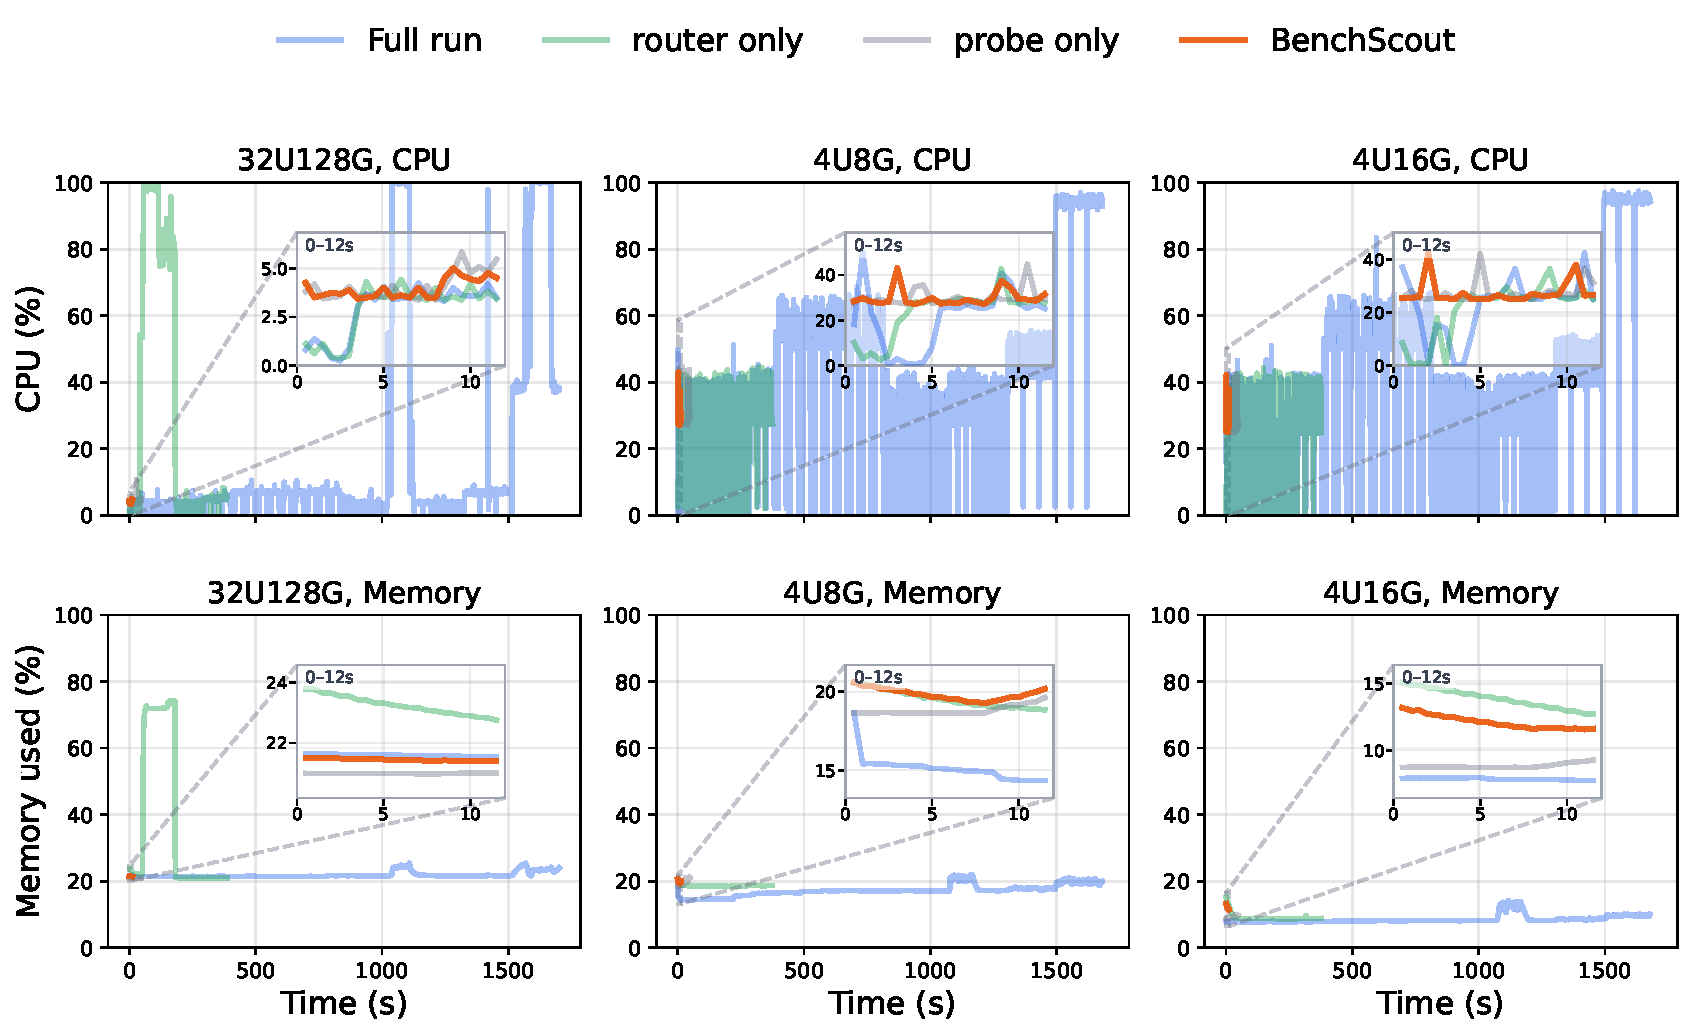
\includegraphics[width=\textwidth]{images/resource_waveforms_2x3_combine.pdf}
    \Description{Six CPU and memory time-series panels compare full UnixBench, router-only, probe-only, and BenchScout runs on M1, M3, and M4; BenchScout activity ends near the start of each full-run trace.}
    \caption{UnixBench CPU and memory waveforms on M1, M3, and M4 ($0.5$\,s sampling).
    Rows: CPU utilization (\%) and memory used (\%); columns: 32U128G, 4U8G, and 4U16G.
    Curves show \emph{Full run}, \emph{router only}, \emph{probe only}, and \emph{BenchScout} on shared axes (${\approx}1680$\,s horizon).
    Dashed guides and per-panel insets magnify $0$--$12$\,s, isolating the early window in which \emph{BenchScout} completes while the full suite remains active for the entire trace.}
    \label{fig:resource-waveforms}
\end{figure*}

\subsection{Model Combination Study}
\label{subsec:model-combination}
The \emph{router only} path isolates the router--reconstructor stack by replacing probe-predicted scores with measured scores.
This removes probe estimation error and tests whether a router-selected subset of true component scores is sufficient to reconstruct the full suite profile.
We exhaustively evaluate all combinations of three routers (LightGBM, MLP, GNN-expert) and three reconstructors (XGBoost, LightGBM, MLP)---nine combinations per suite on M1---under online partial execution plus reconstruction.
Table~\ref{tab:model-combination} reports suite relative error (\%) and benchmark wall-time saved (\%) for UnixBench, \ptscpu{}, and \ptsgpu{}.

The grid reveals that reconstruction is the dominant source of reliability.
Across routers, tree-based reconstructors (XGBoost and LightGBM) are consistently stable, while MLP reconstruction fails catastrophically in several cases, with relative errors far above \(10^{2}\%\).
This is because the reconstructor operates on sparse tabular inputs with structured missingness from Top-\(K\) routing, limited host-local training data, heterogeneous score scales, and nonuniform component correlations.
Boosted trees provide a better inductive bias for this regime: they capture thresholded feature interactions and remain stable under sparse, small-data patterns.
In contrast, MLP reconstructors must learn these conditional imputations from limited masked examples and can extrapolate poorly when the observed subset changes.

We therefore select the best \emph{router only} combinations with tree-based reconstructors on M1: MLP router with LightGBM reconstructor for UnixBench (0.13\% error) and \ptscpu{} (0.22\%), and LightGBM router with LightGBM reconstructor for \ptsgpu{} (1.60\%).
The \emph{router only} supplementary studies in Sections~\ref{subsec:topk-tradeoff} and~\ref{subsec:feature-ablation} reuse these best M1 pairs, while the \emph{probe only} evaluation in Section~\ref{subsec:probe-evaluation} uses independently trained probe regressors.


\begin{table}[t]
\centering
\caption{Router--reconstructor combination study on M1 with online partial execution and reconstruction.}
\label{tab:model-combination}
\small
\setlength{\tabcolsep}{3pt}
\begin{tabular}{l|cc|cc|cc}
\toprule
& \multicolumn{6}{c}{\textbf{Reconstructor}} \\
\cmidrule(lr){2-7}
& \multicolumn{2}{c|}{\textbf{XGB}} 
& \multicolumn{2}{c|}{\textbf{LGBM}} 
& \multicolumn{2}{c}{\textbf{MLP}} \\
\cmidrule(lr){2-3} \cmidrule(lr){4-5} \cmidrule(lr){6-7}
\textbf{Router}
& \textbf{Err.} & \textbf{Save} 
& \textbf{Err.} & \textbf{Save} 
& \textbf{Err.} & \textbf{Save} \\
\midrule
\multicolumn{7}{c}{\textit{UnixBench}} \\
\midrule
LightGBM   & 0.93 & 72.5 & 0.62 & 76.3 & 43.8 & 76.5 \\
MLP        & 0.34 & 78.2 & \textbf{0.13} & 72.1 & 42.8 & 79.1 \\
GNN-expert & 0.28 & 76.5 & 0.42 & 76.5 & 59.0 & 76.5 \\
\midrule
\multicolumn{7}{c}{\textit{\ptscpu}} \\
\midrule
LightGBM   & 0.35 & 74.7 & 7.15 & 60.6 & $1.54{\times}10^{4}$ & 80.2 \\
MLP        & 1.30 & 87.5 & \textbf{0.22} & 89.6 & $2.78{\times}10^{3}$ & 92.3 \\
GNN-expert & 3.12 & 95.5 & 3.14 & 39.6 & $1.65{\times}10^{4}$ & 79.5 \\
\midrule
\multicolumn{7}{c}{\textit{\ptsgpu}} \\
\midrule
LightGBM   & 2.03 & 78.0 & \textbf{1.60} & 78.5 & $3.49{\times}10^{2}$ & 78.5 \\
MLP        & 1.61 & 95.3 & 1.61 & 95.3 & $2.83{\times}10^{2}$ & 95.3 \\
GNN-expert & 1.88 & 95.4 & \textbf{1.60} & 94.9 & $4.03{\times}10^{2}$ & 95.3 \\
\bottomrule
\end{tabular}
\end{table}




\subsection{Probe Model Evaluation}
\label{subsec:probe-evaluation}

This experiment evaluates whether short, time-bounded probes can provide sufficient signal for suite-level performance prediction.
Each component is executed only in micro-probe mode for a fixed budget of 4\,s, optionally collecting eBPF features, and the resulting probe features \(\mathbf{p}_{i,j}\) are used to predict component scores.
Unlike the \ourmethod{} execution pipeline, this experiment does not perform router-based subset selection or reconstruction; instead, it probes every component and directly aggregates the predicted component scores into a suite score.

We train two probe regressors, LightGBM and XGBoost, using probe features collected from each host's historical full runs, and evaluate online prediction against the latest full run on the same host.
For PTS suites, labels use \(\log(1+x)\) scaling with per-profile estimators to handle heterogeneous metric magnitudes.
The evaluation covers UnixBench and \ptscpu{} on all five audited hosts, plus supplied PTS-GPU values for M1 and M6. The repository OOF artifacts cover 11 audited host--suite pairs; the supplied M6 GPU comparison is reported separately.

Table~\ref{tab:probe-models} compares LightGBM and XGBoost on M1 across all three suites.
It reports suite relative error, probe wall time \(T_{\mathrm{partial}}\), full-suite wall time \(T_{\mathrm{full}}\) from the ground-truth run JSON, and the resulting wall-time savings.
On M1, XGBoost consistently achieves lower suite relative error than LightGBM while providing the same wall-time savings, indicating that micro-probes provide useful predictive signal even without selective execution or reconstruction.

\begin{table}[t]
\centering
\caption{Probe model comparison on M1.}
\label{tab:probe-models}
\small
\setlength{\tabcolsep}{2pt}
\begin{tabular}{lccccc}
\toprule
\textbf{Suite} & \textbf{Model} & \textbf{Rel.\ err. (\%)} & $T_{\mathrm{partial}}$ (s) & $T_{\mathrm{full}}$ (s) & \textbf{Saved (\%)} \\
\midrule
\multirow{2}{*}{UnixBench}
 & LightGBM & 0.66 & 48.0 & 319.9 & 85.0 \\
 & XGBoost  & 0.45 & 48.0 & 319.9 & 85.0 \\
\midrule
\multirow{2}{*}{\ptscpu}
 & LightGBM & 2.40 & 52.0 & 13018 & 99.6 \\
 & XGBoost  & 1.03 & 52.0 & 13018 & 99.6 \\
\midrule
\multirow{2}{*}{\ptsgpu}
 & LightGBM & 2.60 & 40.0 & 27018 & 99.9 \\
 & XGBoost  & 2.28 & 40.0 & 27018 & 99.9 \\
\bottomrule
\end{tabular}
\end{table}

These supplementary online probe controls use a separate M1 canonical full run ($T_{\mathrm{full}}=319.9$\,s) from the five-run OOF timing table; the two timing contexts are not directly interchangeable.

\subsection{Top-\(K\) Sweep}
\label{subsec:topk-tradeoff}

Using the best \emph{router only} router--reconstructor pairs on M1 from Section~\ref{subsec:model-combination} (MLP\,+\,LightGBM for UnixBench and \ptscpu; LightGBM\,+\,LightGBM for \ptsgpu), we sweep \(K\) from 1 to 6, capped by each suite's component count.
For each \(K\), the router selects Top-\(K\) experts, partial results are observed, and the reconstructor predicts the suite score.
Evaluation uses within-session random-fold CV on the canonical M1 session (the available fallback because only one session is present), with router checkpoints and reconstructors from the associated \id{trained\_models} directory; reconstructors train on partial subsets of size \(K\). These five-run folds are exploratory and do not provide session-level validation; the reported supplementary analyses should not be read as independent confirmation of the headline model selection.
\begin{figure}[t]
    \centering
    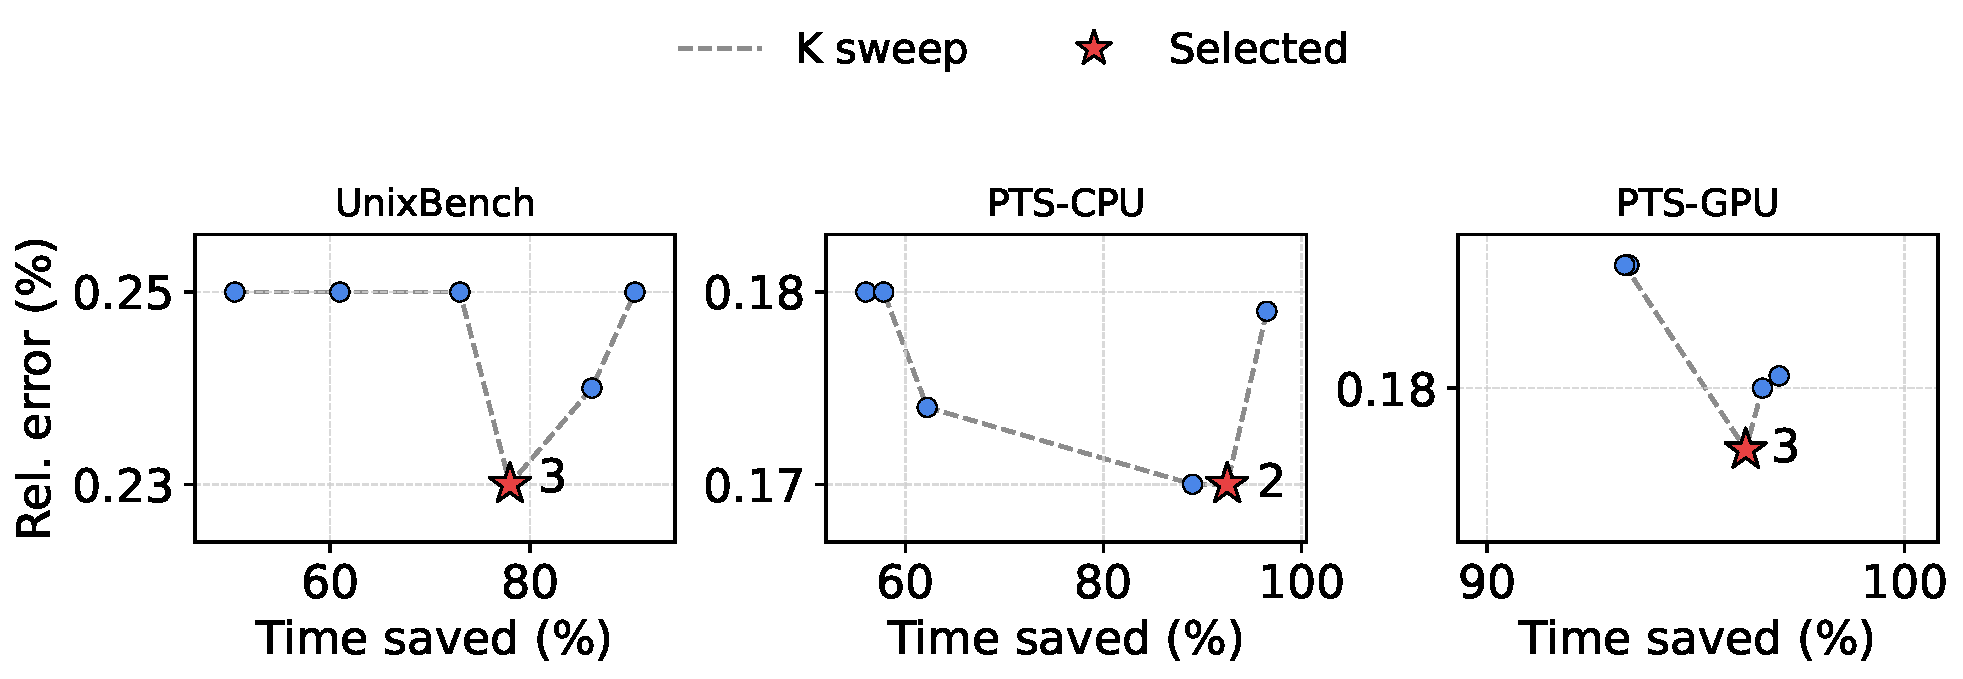
\includegraphics[width=1\linewidth]{images/topk_tradeoff.pdf}
    \Description{Three error-versus-time-saving plots show Top-K trade-offs for UnixBench, PTS-CPU, and PTS-GPU, with selected K values marked.}
    \caption{Top-\(K\) error--saving trade-off using the best router--reconstructor pair for each suite.
    Each point corresponds to a candidate \(K\), with numbers indicating \(K\).
    Stars mark the selected \(K\) according to the balanced score in Equation~\ref{eq:balanced-score}.}
    \label{fig:topk-pareto}
\end{figure}
Figure~\ref{fig:topk-pareto} visualizes the resulting error--saving trade-off, where each point corresponds to one candidate \(K\). Although the figure does not plot the balanced score directly, the selected \(K\) minimizes Equation~\ref{eq:balanced-score}, balancing suite relative error against wall-time savings. On M1, the selected points are at small \(K\): \(K{=}3\) for UnixBench (1.03), \(K{=}2\) for \ptscpu{} (1.01), and \(K{=}3\) for \ptsgpu{} (1.01). These exploratory within-session results show the selected operating points under this score, but do not establish that the router finds generally informative probes or that the chosen \(K\) transfers to new sessions. Increasing \(K\) beyond these points provides limited error reduction in the analyzed folds while reducing estimated time savings.

\begin{table}[t]
\centering
\caption{System-feature ablation at fixed router policy and $K=3$ (offline CV on M1). $\Delta e$ = relative-error change vs.\ complete $\mathbf{x}$ baseline (pp = percentage points; baseline row omitted). Importance rank orders ablated modes by descending $\Delta e$.}
\label{tab:feature-ablation}
\small
\setlength{\tabcolsep}{4pt}
\begin{tabular*}{\columnwidth}{@{\extracolsep{\fill}}l@{\hspace{2pt}}p{0.26\linewidth}ccc@{}}
\toprule
\textbf{Suite} & \textbf{Ablation mode} & \textbf{Rel.\ err. (\%)} & $\Delta e$ (pp) & \textbf{Imp.\ rank} \\
\midrule
\multirow{4}{*}{UnixBench}
 & \id{static\_hw\_only}  & 0.241 & $-$0.003 & 2 \\
 & \id{no\_perf\_pmu}     & 0.243 & 0.000  & 1 \\
 & \id{no\_dynamic\_proc} & 0.241 & $-$0.003 & 3 \\
 & \id{no\_gpu}           & 0.237 & $-$0.007 & 4 \\
\midrule
\multirow{4}{*}{\ptscpu}
 & \id{static\_hw\_only}  & 2.04 & +0.28 & 1 \\
 & \id{no\_perf\_pmu}     & 1.76 & 0.00  & 3 \\
 & \id{no\_dynamic\_proc} & 2.04 & +0.28 & 2 \\
 & \id{no\_gpu}           & 1.75 & $-$0.01 & 4 \\
\midrule
\multirow{4}{*}{\ptsgpu}
 & \id{static\_hw\_only}  & 0.957 & +0.04 & 1 \\
 & \id{no\_perf\_pmu}     & 0.918 & 0.00  & 3 \\
 & \id{no\_dynamic\_proc} & 0.957 & +0.04 & 2 \\
 & \id{no\_gpu}           & 0.818 & $-$0.10 & 4 \\
\bottomrule
\end{tabular*}
\end{table}

\subsection{System Context Feature Ablation}
\label{subsec:feature-ablation}
To quantify which parts of the system context \(\mathbf{x}\) drive reconstruction accuracy, we ablate feature groups while holding router Top-$K$ selection at $K{=}3$ on M1 (leave-one-run-out CV on each suite's canonical session, random-fold fallback), using the same LightGBM reconstructor and \id{trained\_models} checkpoints as in Section~\ref{subsec:topk-tradeoff}.
We compare four ablated modes against a complete-\(\mathbf{x}\) baseline (not shown):
\id{static\_hw\\\_only} (hardware topology, memory, cache, and GPU inventory; zero dynamic/PMU),
\id{no\_perf\_pmu} (remove PMU-derived rates except \id{perf\_event\_paranoid}),
\id{no\_dynamic\_proc} (remove load, fault, and bandwidth-proxy dynamics),
and \id{no\_gpu} (remove GPU/OpenCL dimensions).
Table~\ref{tab:feature-ablation} reports mean out-of-fold suite relative error and $\Delta e_m$ relative to the complete-\(\mathbf{x}\) baseline.
Importance rank (1 = most important to keep among the four ablated groups) sorts ablated modes by descending $\Delta e_m$.
On \ptscpu, ablating static hardware or dynamic \path{/proc} proxies increases error by ${\approx}0.28$~pp; PMU and GPU groups have smaller effects.
On UnixBench all $\Delta e_m$ magnitudes stay below $0.01$~pp on M1.
On \ptsgpu, removing GPU/OpenCL inventory features lowers error by 0.10~pp. In this small replay, those features add noise rather than useful signal; the result cautions against treating hardware descriptors as uniformly beneficial inputs.


\subsection{Robustness to Probe-Telemetry Restrictions}
\label{subsec:probe-ebpf-ablation}

Section~\ref{subsec:time-bounded-probing} and Appendix~Table~\ref{tab:feature_collection} include optional eBPF-derived scheduling and syscall rates in the in-run probe vector~\(\mathbf{p}_{i,j}\).
These signals can improve observability on permissive systems, but they should not become a deployment prerequisite.
In restricted environments where bpftrace is unavailable or tracing privileges are denied, \ourmethod{} treats eBPF features as optional telemetry: it sets the \id{ebpf\_available} flag to zero and zero-masks the corresponding probe dimensions instead of aborting the probe or changing the feature layout.
This design preserves a deterministic input schema while allowing the model to fall back to the remaining context and probe signals.
\begin{table}[t]
\centering
\caption{eBPF degradation on M1 UnixBench \emph{Probe only} (LightGBM; $D{=}4$\,s; $Y{=}3185.5$). \textbf{sched}: mean context-switch rate ($10^4$/s).}
\label{tab:probe-ebpf-ablation}
\small
\begin{tabular*}{\columnwidth}{@{\extracolsep{\fill}}lrrrrrr@{}}
\toprule
\textbf{Telem.} & \textbf{Err (\%)} & $|\hat{Y}{-}Y|$ & $\hat{Y}$ & $T_{\mathrm{pr}}$ (s) & \textbf{eBPF ok} & \textbf{sched} \\
\midrule
On  & 0.27 & 8.48 & 3194.0 & 61.8 & 12/12 & 8.3 \\
Off & 0.17 & 5.42 & 3190.9 & 60.6 & 0/12 & --- \\
\bottomrule
\end{tabular*}
\end{table}

To evaluate robustness under realistic telemetry restrictions, we conduct a controlled \emph{Probe only} experiment on M1 (32U128G) with UnixBench in which eBPF tracing is unavailable after training. We fix the trained M1 LightGBM probe regressor under the micro-probe setting (4\,s per component) and run two back-to-back online conditions on the same host:
\textbf{(i)~eBPF on}, where bpftrace is enabled with elevated privileges; and
\textbf{(ii)~eBPF off}, where tracing is disabled and all eBPF dimensions are zero-masked.
Each condition probes all 12 UnixBench components, predicts subtest indices, aggregates the suite score, and compares against the latest full-run ground truth in the canonical session (\(Y=3185.5\)).
The probe regressor is trained on M1 historical runs using the same micro-probe protocol and eBPF-enabled feature collection.

Table~\ref{tab:probe-ebpf-ablation} shows that both conditions completed with sub-percent error, but zero-masking eBPF produced the lower error in this single run (0.17\% versus 0.27\% with eBPF available); probe times were comparable (60.6\,s versus 61.8\,s).
Thus, this observation supports graceful operation when tracing is unavailable, not an accuracy benefit from eBPF. It does not establish end-to-end robustness across hosts, suites, contention levels, or other telemetry failures.


\subsection{Probe Duration Sensitivity}
\label{subsec:probe-duration-sensitivity}

Section~\ref{subsec:time-bounded-probing} fixes a per-component probe budget as the primary knob for \emph{Probe only} latency versus fidelity.
We quantify this accuracy--cost frontier on M1 (32U128G) with a controlled UnixBench \emph{Probe only} sweep over $D \in \{2,4,8\}$\,s: for each duration, we collect micro-probes for all 12 components and train a dedicated LightGBM regressor (eBPF off to isolate duration effects) before online evaluation against the latest full run ($Y{=}3185.5$, $T_{\mathrm{full}}{=}319.9$\,s).
Table~\ref{tab:probe-duration-sensitivity} reports suite relative error and wall-time savings for each~$D$; all 12 probes complete without timeout or pipeline failure.
Error decreases monotonically with~$D$ while probe cost scales roughly linearly in $D{\times}12$. At $D{=}4$\,s, suite error is 0.56\% with ${\approx}81\%$ wall-time saved, balancing accuracy against the 0.44\% error at $D{=}8$\,s and the lower probe cost at $D{=}2$\,s (0.80\%, 88.6\% saved).
This confirms the 4\,s default used in Section~\ref{subsec:probe-evaluation} and the eBPF degradation study (Section~\ref{subsec:probe-ebpf-ablation}).

\begin{table}[t]
\centering
\caption{Probe duration sweep on M1 UnixBench \emph{Probe only} (LightGBM; micro; eBPF off; $Y{=}3185.5$, $T_{\mathrm{full}}{=}319.9$\,s).}
\label{tab:probe-duration-sensitivity}
\small
\begin{tabular*}{\columnwidth}{@{\extracolsep{\fill}}rrrrrrr@{}}
\toprule
$D$ (s) & \textbf{Err(\%)} & $|\hat{Y}{-}Y|$ & $\hat{Y}$ & $T_{\mathrm{pr}}$ (s) & \textbf{Saved(\%)} & \textbf{Probe-ok} \\
\midrule
2 & 0.80 & 25.4 & 3210.9 & 36.4 & 88.6 & 12/12 \\
4 & 0.56 & 17.8 & 3203.3 & 60.4 & 81.1 & 12/12 \\
8 & 0.44 & 13.9 & 3199.4 & 108.6 & 66.1 & 12/12 \\
\bottomrule
\end{tabular*}
\end{table}


\subsection{Selective-Execution Baselines}
\label{subsec:selective-execution-baselines}
The following M1 replay compares additional same-$K$ policies and reconstruction methods omitted from the cross-host headline table. The rows do not all receive identical information: BenchScout uses its probe-imputed selected scores, while correlation and matrix completion use their respective replay inputs, and the adaptive-probing result comes from a separately configured within-session experiment. We report them to expose the quality range of simple and structured alternatives, not as a single controlled ranking.

\begin{table}[t]
\centering
\caption{Additional M1 UnixBench selective-execution baselines ($K=3$, within-session five-fold replay). Inputs and timing protocols differ by method; this table supplements, rather than replaces, the matched router controls in Table~\ref{tab:matched-routing}.}
\label{tab:m1-strong-baselines}
\small
\setlength{\tabcolsep}{4pt}
\begin{tabular}{lrr}
\toprule
\textbf{Method} & \textbf{Mean err. (\%)} & \textbf{P95 err. (\%)} \\
\midrule
BenchScout full pipeline & 0.180 & -- \\
Fixed first-$K$ subset & 0.244 & -- \\
Random-$K$ subset & 0.236 & -- \\
Correlation reconstruction & 0.770 & 0.928 \\
Matrix completion & 0.503 & 0.795 \\
Adaptive probing & 0.072 & 0.259 \\
\bottomrule
\end{tabular}
\end{table}

The $0.072\%$ adaptive-probing row is numerically stronger than the 0.180\% headline M1 value, which prevents a broad claim that the full pipeline is best on this host. It is a distinct replay protocol and should motivate a controlled follow-up rather than be hidden or treated as directly interchangeable.

\section{Related Work}
\subsection{Performance Evaluation}
Operating-system suites such as LMbench, UnixBench, and HBench-OS support robustness and embedded-system studies~\cite{brown1997operating,smith2011byte,hatt2007benchmarking,koopman1997comparing,kanoun2006dependability,garre2014performance,watfa2014benchmarking,silva2019operating}. Cost reduction includes suite selection, execution-time prediction, and adaptive stopping~\cite{Infantolino2014SelectingBenchmark,Saavedra1996AnalysisBenchmark,Mittal2023AdaptiveStopping}. BenchScout estimates omitted entries of a specified profile from bounded target-host probes, comparing full-run, history, and fixed-subset baselines; its router ranks components by predicted score. Application suites and Web studies cover scale-out behavior, tuning, sampled-run models, and cloud search~\cite{ferdman2012clearing,gan2019deathstarbench,chung2004webtuning,venkataraman2016ernest,alipourfard2017cherrypick,voegele2018wessbas}. Our Web endpoint reconstructs a five-load curve from three target measurements; fixed single-load controls match all throughput-only winners, so no tuning-benefit claim is made. The UnixBench aggregate is published and the PTS aggregate is a paper-defined log-mean proxy (Section~\ref{subsec:aggregator}).

\subsection{Performance Prediction}
\label{subsec:rw-performance-prediction}
Prior work lowers evaluation cost by predicting performance instead of measuring it.
Simulation- and regression-based methods estimate unexplored design points from a fraction of simulated configurations~\cite{ipek2005approach,ipek2006efficiently,lee2006accurate,sharkawi2009performance}; analytical models derive performance from explicit processor mechanisms such as pipeline stalls, cache misses, prefetching, and MSHR limits~\cite{hartstein2002optimum,eyerman2009mechanistic,chen2011hybrid,eyerman2011mechanistic,van2015micro}; and machine-learning models map program or hardware features to runtime or power on another platform (e.g., XAPP, LACross) or to new CPUs from public specifications~\cite{ardalani2015cross,zheng2016accurate,wang2019predicting,tousi2022comparative}.
These approaches estimate unmeasured points from simulation or static features. BenchScout instead uses bounded target-host probes; its aggregate is the published UnixBench index or the paper-defined PTS proxy.

\section{Limitations and Reproducibility}
\label{sec:limitations}
The system-suite evaluation uses host-specific models and run-held-out folds within one five-run session per host--suite; it does not establish future-day or unseen-host generalization. The Web study uses one host, four strict CloudSuite sessions per PHP-FPM setting (one failed session is sensitivity-only), and four randomized Nginx blocks, so it does not establish production validity.

The Web endpoint is profile fidelity: fixed single-load controls match all eight throughput-only winners, so no tuning-decision advantage is claimed. CloudSuite applies the same compression endpoint to offered-load coordinates; the component-suite path uses benchmark-component routing and probe-score prediction. Workload-specific latency screens are reported separately from profile accuracy.

System-suite probe budgets use historical full-run durations rather than paired end-to-end timings. The four isolated FPM4 pairs mix 60/120-second and matched 60/60-second full-first cells; ordering, drift, and $n=4$ still prevent probe-count causal claims. Two concurrent full-first stress sessions had 31.58--41.89\% omitted-load error and are reported separately; session 10 is excluded for invalid operation mix. CloudSuite costs are reconstructed, partial FPM8 sessions are excluded, PTS uses a paper-defined proxy, and the M6/T4 GPU case lacks run-level logs (Appendix~\ref{app:artifact-notes}).

\section{Conclusion}

We study compressing cloud-infrastructure evaluation with bounded target measurements. UnixBench reaches 0.21\% median error at an estimated 18.1\,s context-plus-probe budget, while omitted-component MAPE is 0.88\% for UnixBench and 2.29\% for PTS-CPU. In CloudSuite's coordinate-specific cold-start profile recovery, three measurements reduce unselected-load MAPE from 39.16\% for history-only to 8.74\% with interpolation. Four isolated FPM4 pairs ($n=4$) show 5.18--19.93\% omitted-load MAPE and 5.28--19.45\% full-curve MAPE; probe phase totals range from 472.638 to 545.056\,s and full-reference phase totals from 792.409 to 1,093.760\,s. Concurrent stress sessions expose higher error and are reported separately. The evidence supports measurement compression under the audited operating conditions: accuracy is retained for the reported folds and targets while the new measurement phase is bounded, with history and fixed policies exposed as credible alternatives.


\clearpage
\bibliographystyle{acm}
\bibliography{sample-base}
\clearpage
\appendix
\section{Feature Collection Inventory}
\label{app:feature-collection}

Table~\ref{tab:feature_collection} lists representative pre-run context and in-run probe signals.

\begin{table*}[t]
\centering
\caption{Purpose-oriented feature groups organized by collection stage. Pre-run signals form the system context \(\mathbf{x}_i\), while in-run probe signals form the probe vector \(\mathbf{p}_{i,j}\).}
\label{tab:feature_collection}
\small
\setlength{\tabcolsep}{5pt}
\renewcommand{\arraystretch}{1.10}
\begin{tabular}{p{0.07\linewidth}| p{0.15\linewidth} p{0.29\linewidth} p{0.42\linewidth}}
\toprule
\textbf{Stage} & \textbf{Signal type} & \textbf{Purpose} & \textbf{Representative signals} \\
\midrule

\multirow{3}{=}{Pre-run}
& Static host profile
& Identify stable host configuration.
& CPU topology, NUMA layout, memory size, gcc versions \\

& System pressure
& Capture transient pre-run load.
& CPU/GPU utilization, iowait, load average, runnable tasks \\

& PMU / perf
& Profile microarchitectural behavior.
& IPC, cycles/s, instructions/s, cache/branch miss ratios \\

\midrule

\multirow{5}{=}{In-run}
& Probe progress
& Record observed benchmark progress.
& Configured probing duration, elapsed wall-clock time \\

& eBPF-based tracing
& Observe prefix-level kernel activity.
& Scheduling-switch rate, syscall-entry rate, eBPF availability \\

& Resource usage
& Summarize prefix resource usage.
& User/system/idle CPU ratio, minor faults, major faults \\

& Workload identity
& Provide workload semantic context.
& CPU, memory, I/O, thread, syscall, GPU category \\

& Probe flags
& Mark probe mode and failures.
& Micro workload flag, real-component flag, timeout flag \\

\bottomrule
\end{tabular}
\end{table*}

\section{Artifact and Transfer Notes}
\label{app:artifact-notes}
The anonymous bundle contains raw CPU/UnixBench records, source, saved models, HTTP logs, and audited split/output JSON. It includes the M1 router--reconstructor grid, per-run feature ablations, waveforms, and scripts for the HTTP, transfer, and feature-use analyses. The model grid and feature ablations reuse the five-run session; complete command provenance is unavailable for some legacy tables.

The strict CloudSuite split audit is the session-audit JSON under the round-8 results directory; its input hash prefix is \texttt{ff3bc3c19b75} (full SHA256 is stored in the artifact). Session 5 also contains paired per-cell phase timings: probe/full totals are 790.86/1,119.02\,s for FPM4 and 795.10/1,094.00\,s for FPM8 across five loads. Sessions 6, 8, 9, and 14 contain the four valid exploratory FPM4 accuracy/cost pairs summarized in Table~\ref{tab:cloudsuite-paired-fpm4}; sessions 9 and 14 use matched 60-second cells and full-first order. Session 10 has timing provenance (probe/full 479.122/787.639\,s) but its full-scale20 operation mix is invalid and it is excluded from accuracy replication. All valid sessions use the pre-fixed evenly spaced interpolation policy with probe loads 20/60/100 and full-reference loads 20/40/60/80/100. Session 9 records are under \path{round-8-cloudsuite/results/bsr8-local-supplemental-session9-20261014T030226Z-1034987}; session 10 records are under \path{round-8-cloudsuite/results/bsr8-local-supplemental-session10-20261014T032440Z-1155738}; session 14 records are under \path{round-8-cloudsuite/results/bsr8-local-supplemental-session14-20261014T054819Z-2356052}. Timings include fresh service reset/setup per cell and are not selective single-deployment end-to-end runs. Partial FPM8 session-6 and session-7 provenance is retained but excluded. The artifact includes raw records and the omitted-component audit with exact run and fold joins.

\begin{comment}
\section{Supplementary Baseline Tables}
\label{app:supplementary-baselines}
The selective-execution, HTTP, tail-latency, temporal-transfer, GPU case-study, and oracle results are presented with their corresponding analyses in the main text. This appendix retains artifact provenance only.

\begin{table}[t]
\centering
\caption{Held-out HTTP profile MAPE across eight configuration-block profiles (four blocks, two configurations). The random row averages the ten possible $K=3$ subsets within each profile. Each probe policy uses three 4-second observations; cost is nominal $\texttt{wrk}$ time, while history mean uses no new probes.}
\label{tab:http-profile-baselines-appendix-copy}
\scriptsize
\setlength{\tabcolsep}{2pt}
\begin{tabular*}{\columnwidth}{@{\extracolsep{\fill}}p{0.42\columnwidth}rr@{}}
\toprule
\textbf{Policy} & \textbf{Throughput MAPE (\%)} & \textbf{Probe s} \\
\midrule
History mean & 1.395 & 0 \\
Fixed first three & 2.530 & 12 \\
Fixed middle three & 2.792 & 12 \\
Uniform random $K=3$ & 2.910 & 12 \\
Nested train-only $K=3$ & 2.119 & 12 \\
\bottomrule
\end{tabular*}
\end{table}

\section{Nginx Tail-latency Diagnostics}
\label{app:nginx-p99}
Table~\ref{tab:http-p99-baselines} gives the descriptive p99 curve errors for the static-content Nginx counterexample. The profile is based on a small number of successful operations per load; these errors are not a production tail-latency guarantee.
\begin{table}[t]
\centering
\caption{Descriptive held-out p99 curve MAPE for the static-content Nginx counterexample.}
\label{tab:http-p99-baselines-appendix-copy}
\small
\begin{tabular}{lr}
\toprule
\textbf{Policy} & \textbf{p99 MAPE (\%)} \\
\midrule
History mean & 14.024 \\
Fixed first three & 27.809 \\
Fixed middle three & 30.113 \\
Uniform random $K=3$ & 40.186 \\
Nested train-only $K=3$ & 29.625 \\
\bottomrule
\end{tabular}
\end{table}

\paragraph{Single-run M1 temporal diagnostic.} On 2026-10-12, saved checkpoints from June 10 or earlier predicted 3189.654 for a newly collected full UnixBench run on M1 (target 3418.5; 6.6943\% error, $n=1$). Router scores tied across all 12 subtests, so selection fell back to the first three listed components: \id{dhry2reg}, \id{whetstone-double}, and \id{execl}. Context collection took 8.699\,s; the three probes, each capped at 4\,s, took 3.012\,s total. This single observation is descriptive only. Checkpoints saved with scikit-learn 1.8.0 were loaded under 1.7.2, producing compatibility warnings. The reported 319.9\,s sum of component durations is not an end-to-end full-run time.

\paragraph{Offline whole-host diagnostic.} An outer leave-one-host-out replay excluded each test host from router, probe-model, and reconstructor fitting; source-host reconstructor inputs used inner host-held-out probe fits. Test-host probes are archived telemetry from full-run collections, so this is offline transfer analysis rather than a fresh online experiment. The four policies average 15.07\% mean host error and 40.44\% worst-host error, with mean errors within 0.002 percentage points of one another. Predicted suite indices differ by at most 0.079 points over the 25 runs. This diagnostic does not validate fresh probe collection or online transfer.

\begin{table}[t]
\centering
\caption{Online PTS-GPU case studies on M1 and M6; bold marks the lowest reported error per host. The 15\,s entries denote selected-probe time, not end-to-end cost (M1 context collection adds 7.93\,s). M1's target overlaps the model-selection corpus, and M6 run-level logs are unavailable; these results are descriptive and separate from the M1 cross-validation in Table~\ref{tab:pts-gpu-audited}. Full-suite times sum profile durations.}
\label{tab:gpu-provenance-appendix-copy}
\footnotesize
\setlength{\tabcolsep}{4.5pt}
\begin{tabular}{llcc|cc}
\toprule
\multirow{2}{*}{\textbf{Suite}} & \multirow{2}{*}{\textbf{Method}} & \multicolumn{2}{c|}{\textbf{M1 (RTX 3090 Ti)}} & \multicolumn{2}{c}{\textbf{M6 (T4)}} \\
\cmidrule(lr){3-4} \cmidrule(lr){5-6}
& & \textbf{Err. (\%)} & \textbf{Cost (s)} & \textbf{Err. (\%)} & \textbf{Cost (s)} \\
\midrule
\multirow{4}{*}{\ptsgpu}
& Full-suite & -- & 27018.0 & -- & 12951.0 \\
& Wang-style DNN proxy & 0.26 & 3.5 & 5.13 & 3.5 \\
& Tousi-style MLP proxy & 98.85 & 3.5 & 67.14 & 3.5 \\
& \ourmethod & $\mathbf{0.18}$ & 15.0 & $\mathbf{0.14}$ & 15.0 \\
\bottomrule
\end{tabular}
\end{table}

The M1 online JSON records target \texttt{run-05.json}, prediction 239.5497
against target 239.9724 (0.1761\% relative error), 15.035\,s selected-probe
time, 7.930\,s context collection, and 22.965\,s total hybrid wall time.
However, the selected router checkpoint came from a grid trained/evaluated on
all five archived runs, including run-05. This is a traceable single online
report, not an independent held-out estimate, and it must remain separate from
the 0.9534\% run-held-out result in Table~\ref{tab:pts-gpu-audited}.
The source for the M6/T4 row is still unavailable, so that row remains
unverified provenance.

An offline leave-one-host-out oracle test used held-out \emph{full-run
component scores}. The training-host score-ranked subset had 4.49\% mean error
(0.98--10.25\% across hosts), versus 9.53\% random, 12.57\% first-three,
16.26\% context-only Ridge, and 22.60\% training mean. This supports only the
utility of observed target-host components: oracle scores do not validate
routing, short probes, or online transfer, and subset choice remained
host-sensitive.

\end{comment}
\end{document}
\endinput
%%
%% End of file `sample-sigconf.tex'.
